\chapter{Implementierung}
\label{ch:Implementierung}

	\section{Schlupfregelung}
			\label{sec:Schlupfregelung}
			
			Um die in Kapitel \ref{sec: Reglung und autonomes Fahren} beschriebenen Probleme im Anlaufverhalten des ALF
			entgegenzuwirken wird zusätzlich zur im MCM bereits bestehenden Drehmomentregelung
			eine übergeordnete Drehzahlregelung implementiert. Um das Systemverhalten der vorhandenen Antriebe zu analysieren wird eine Sprungantwort aufgenommen,
			indem eine maximale Drehmomentanforderung an die Motorcontroller
			gesendet und die resultierenden Drehzahlen der Motoren aus dem
			CAN-Bus ausgelesen wird.
			
			
				\begin{figure}[H]
				\centering
				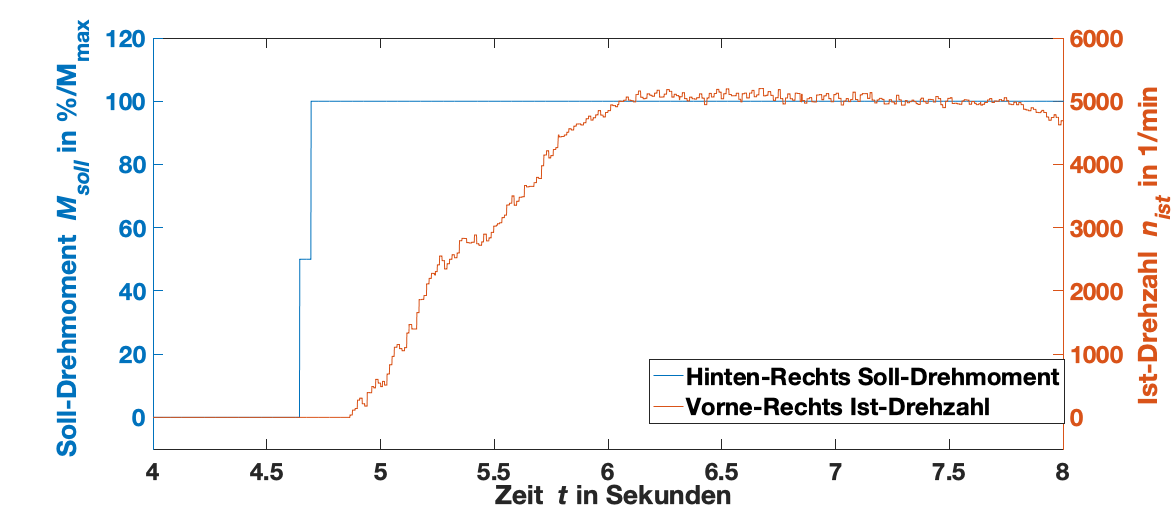
\includegraphics[width=0.8\textwidth]{Bilder/sprungantwort.png}
				\caption{Sprungantwort des Motors hinten rechts}
				\label{fig: Sprungantwort des Motors hinten rechts(BR)}
			\end{figure} 
			
			Anhand der Sprungantwort aus Abbildung \ref{fig: Sprungantwort des Motors hinten rechts(BR)}, lässt sich das Verhalten eines Verzögerungsgliedes 2. Ordnung identifizieren, dessen Übertragungsfunktion mit der allgmeinen Form 
			
			\begin{equation}
					G(s)=\frac{k_s}{T^2s^2+2DTs+1}
					\label{eq:pt2}
			\end{equation}\newline
			beschrieben wird \cite{unbehauen,lunze}. Durch diese Identifikation kann mithilfe der Matlab Funktion Transfer Function Estimation (tfest) eine Übertragungsfunktion für die Sprungantwort aus Abbildung \ref{fig: Sprungantwort des Motors hinten rechts(BR)} geschätzt werden \cite{tfest}. Für die Anwendung von tfest sind Kenntnisse über die Pol- und Nullstellen der Übertragungsfunktion erforderlich. Bei einem Verzögerungsglied 2. Ordnung treten aufgrund der Gebrochen-Rationalen Funktion aus Gleichung \ref{eq:pt2} zwei Polstellen und keine Nullstelle auf \cite{unbehauen}. Durch Anwenden der Funktion tfest erhält man die Übertragungsfunktion: 
			
			\begin{equation}
			G(s)=\frac{248.7}{s^2+3.074s+5.101}\text{.}
			\label{eq:tfestpt2}
			\end{equation}\newline
			Eine Simulation zur Verifikation der approximierten Übertragungsfunktion in Simulink, mit den gleichen Simulationsparametern wie bei der Aufnahme der Sprungantwort, liefert ein äquivalentes Übertragungsverhalten der geschätzten und experimentell ermittelten Sprungantwort und ist in der Abbildung \ref{fig: transfer estimate} zu sehen.
			 
			 \begin{figure}[H]
			 	\centering
			 	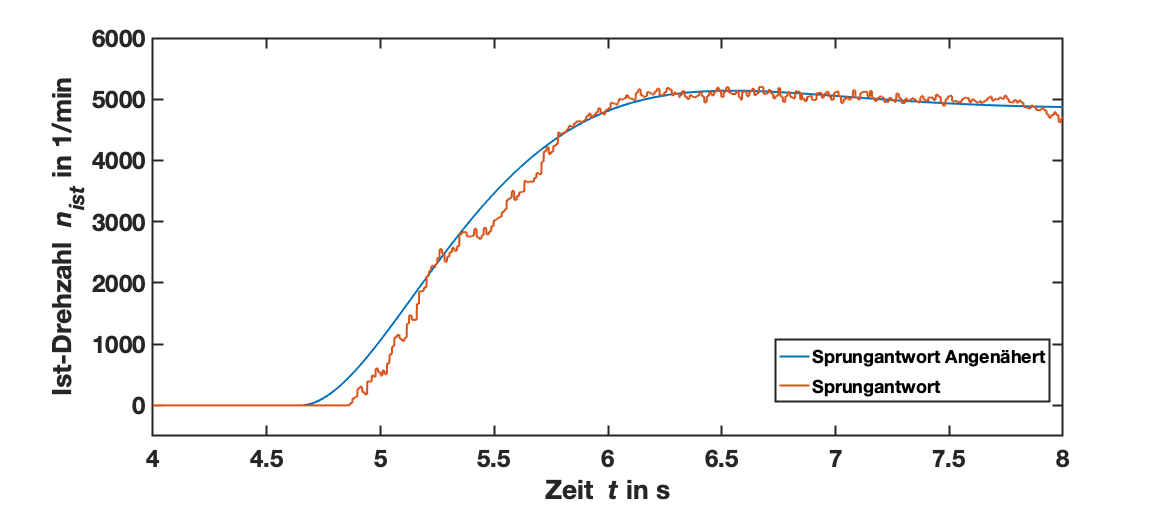
\includegraphics[width=0.8\textwidth]{Bilder/sprungantwort_estimate.png}
			 	\caption{Mit tfest geschätzte Sprungantwort (blau) und experimentell ermittelte Sprungantwort(orange) übereinander gelegt.}
			 	\label{fig: transfer estimate}
			 \end{figure}
		 
			Die Übertragungsfunktion wird in die Form aus Gleichung \ref{eq:pt2} umgestellt, sodass die Zeitkonstante und Dämpfung bestimmt werden kann. 
			%Das Zerlegender Übertragungsfunktion in zwei Pt1 Glieder um einen Regler mit demBetragsoptimum auszulegen ist in diesem Fall nicht möglich, da die Funktionzwei konjuiert Komplexe Pole mit negtivem Realteil aufweist.
			 
			 \begin{equation}
			 G(s)=\frac{48.7551}{0.1815s^2+0.6026s+1} \text{ daraus folgt } D=0.7071 \text{ und } T=0.4261s
			 \label{eq:tfestpt2}
			 \end{equation}\newline			
			 
			Das nun vorhandene mathematische Modell der Übertragungsfunktion kann genutzt werden um verschiedene Regler in Matlab/Simulink zu simulieren und anschließend am ALF zu implementieren.
			
			
		\subsection{Drehzahlregelung}
		\label{sec: Drehzahlregelung}
		
		Die Drehzahlregelung wird mithilfe eines PI-Reglers realisiert, da dieser die Vorteile eines P- und I-Reglers vereint \cite{praktischeregelungstechnik}. Aufgrund des P-Anteils, reagiert der Regler unmittelbar und hat durch die zeitliche Integration der Regelabweichung keine bleibende Regeldifferenz. Durch das vorhandene mathematische Modell können verschiedene PI-Regler an der Regelstrecke simuliert werden. Es werden mehrere PI-Regler mit den Einstellregeln nach Chien, Hrones und Reswick und empirisch am Fahrverhalten ausgelegt und simuliert. Für die Einstellregeln sind Informationen über die Verzugszeit ($T_{u}$) und die Anstiegszeit ($T_{g}$) notwendig, diese Größen werden durch die Anwendung des  Wendetangentenverfahrens an der approximierten Regelstrecke gewonnen. \cite{unbehauen,praktischeregelungstechnik}
		
			\begin{figure}[H]
			\centering
			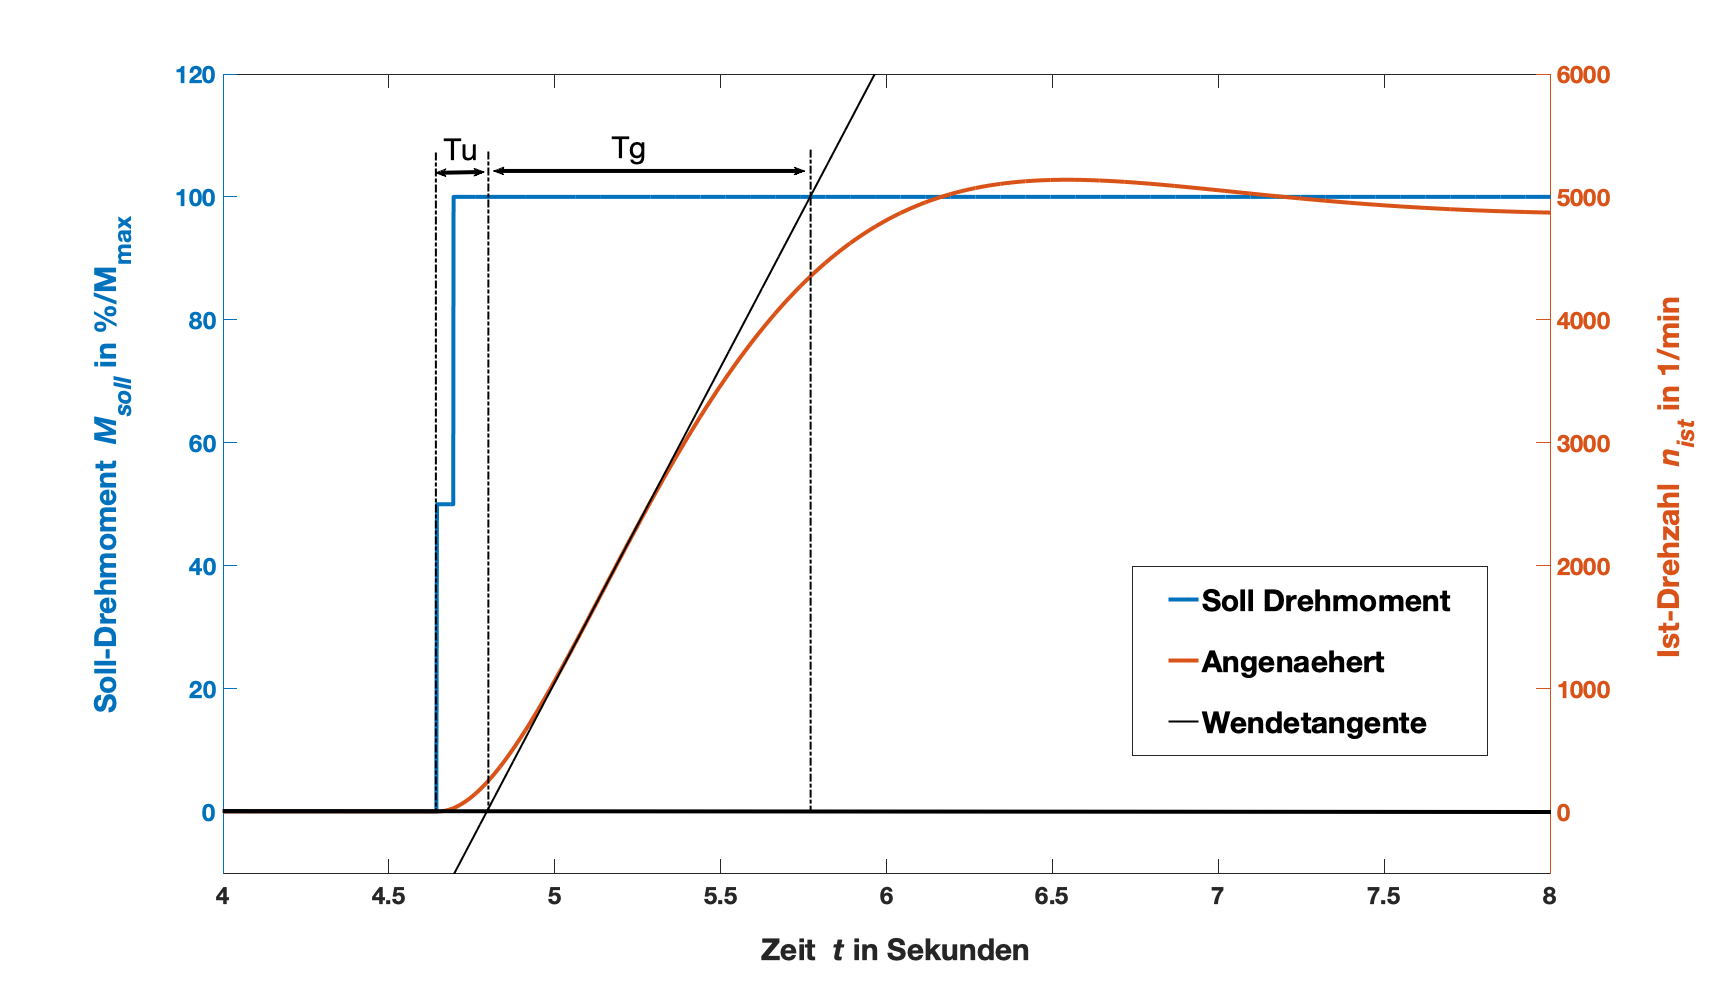
\includegraphics[width=1.0\textwidth]{Bilder/sprungantwort_wende.png}
			\caption{Sprungantwort mit Wendetangente für die Zeitkonstanten $T_{u}$ und $T_{g}$}
			\label{fig: sprungantwort_wende}
			\end{figure} 
		
		
			Mithilfe der in Abbildung \ref{fig: sprungantwort_wende} eingezeichneten Wendetangente können die Zeitkonstanten bestimmt werden, welche nötig sind um die Nachstellzeit $T_n$ und Verstärkung $K_P$ für den PI-Regler zu bestimmen. Durch eine Aktualisierung des Bewegungsziels wird die Führungsgröße geändert. Aufgrund der sich ändernden Führungsgröße und einer Dämpfung der Übertragungsfunktion von $D=0.7071$, wurden die Einstellregeln für Führungsverhalten mit $D \approx 1 $ mit 0\% Überschwingen und $D \approx 0.45 $  mit 20\% Überschwingen gewählt \cite{praktischeregelungstechnik}. Die Gleichungen \ref{eq: gpi1}, \ref{eq: gpi2} und \ref{eq: gpi3} zeigen die ermittelten Regler, nach den Einstellregeln von Chien, Hrones und Reswick, sowie den empirisch, durch Beobachtung des Fahrverhaltens, entwickelten Regler.
		
			\begin{align}
			\label{eq: gpi1}
			G_{pi1}(s) &= \frac{0.07403s+0.07793}{0.9499s}\\\nonumber\\
			\label{eq: gpi2}
			G_{pi2}(s) &= \frac{0.0582s+0.04546}{1.14s}\\\nonumber\\
			\label{eq: gpi3}
			G_{pi2}(s) &= \frac{0.1s+0.005}{s}
			\end{align}
		
	
			Die Simulation mit den drei Reglern $G_{pi1}(s)$, $G_{pi2}(s)$ und $G_{pi3}(s)$ an der approximierten Regelstrecke aus Gleichung \ref{eq:tfestpt2}, ergibt die in Abbildung \ref{fig: simulation_regler} dargestellten Regelverläufe der drei Regelkreise. Dabei ist eine deutliche Regeldifferenz bei dem empirisch ermittelten Regler zu beobachten. Da dieses Verhalten nicht den im Lastenheft erhobenen Anforderungen an die Regelung entspricht, ist dieser Regler nicht für eine Implementierung in dem ALF geeignet.

					\begin{figure}[H]
				 	\centering
				 	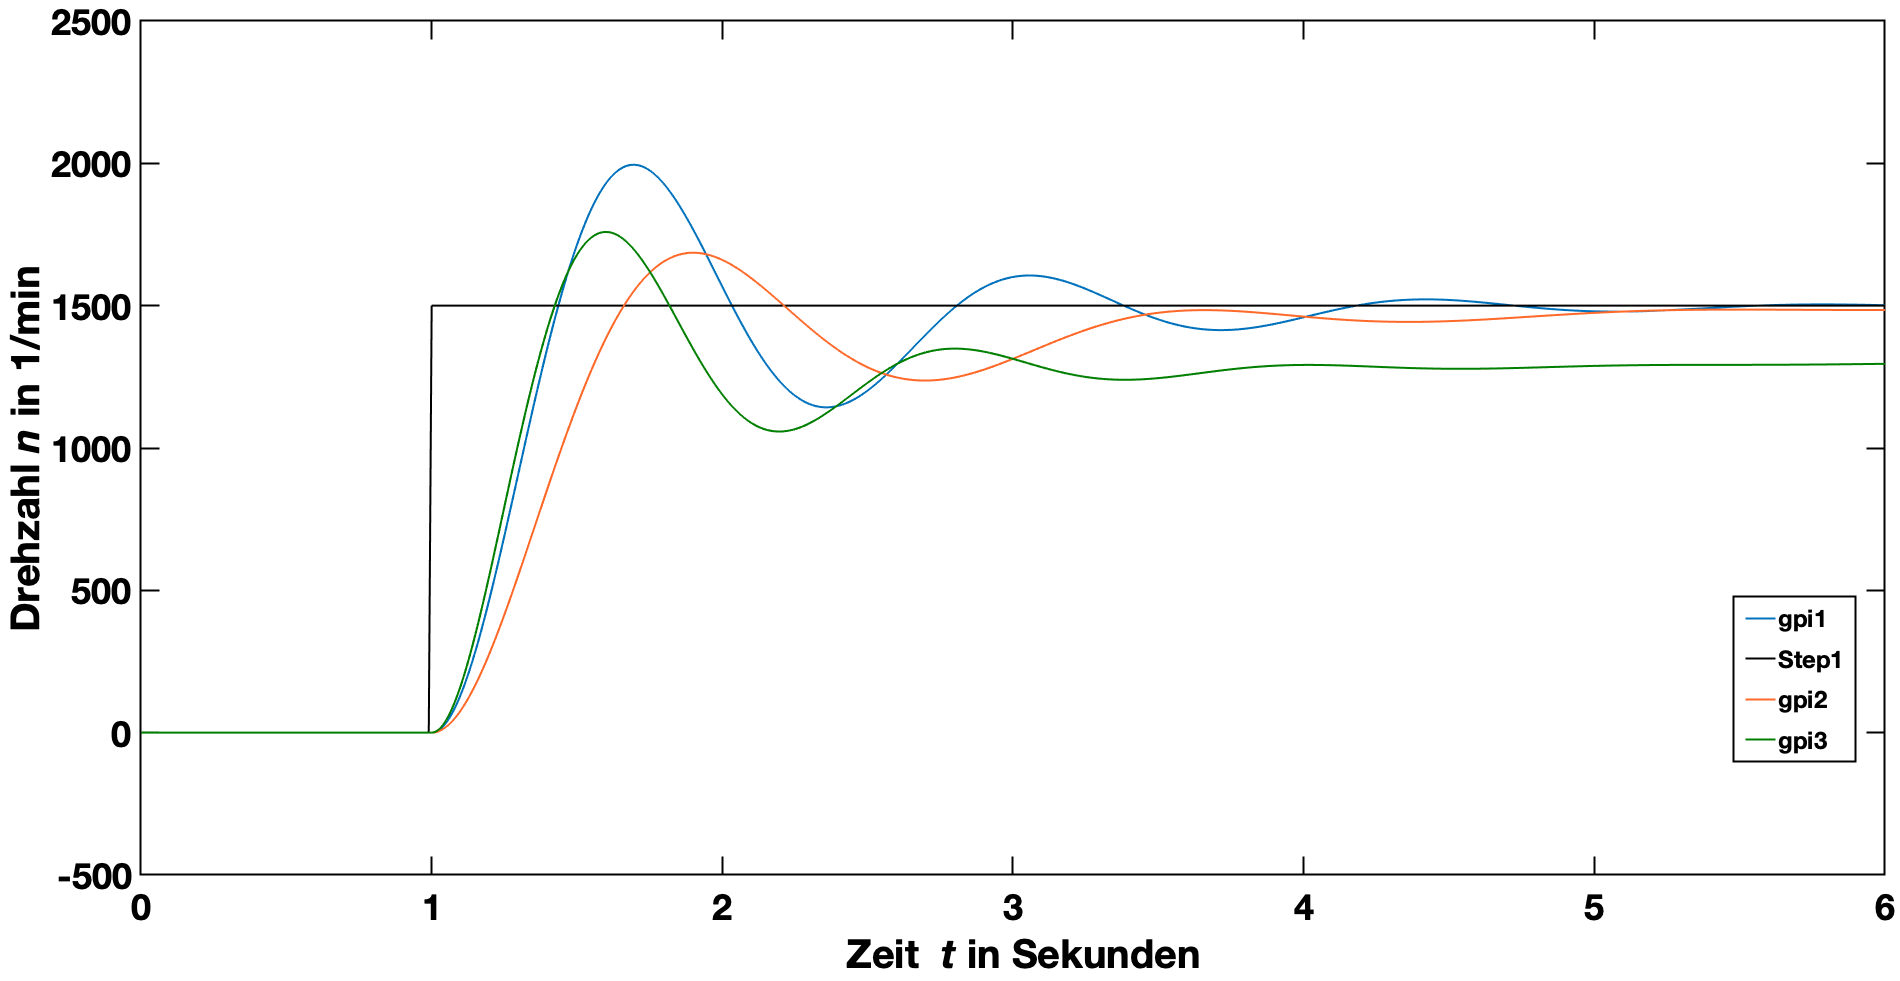
\includegraphics[width=1.0\textwidth]{Bilder/simulation_regler.png}
				 	\caption{Regelverläufe für die Regler aus Gleichung \ref{eq: gpi1}, \ref{eq: gpi2} und \ref{eq: gpi3}}
				 	\label{fig: simulation_regler}
				 	\end{figure} 
			
			Die Implementierung des Reglers im ALF erfolgte mit einem LTI-System aus der Control System Toolbox von Matlab/Simulink, wobei die übergeordnete Winkelregelung aus Kapitel \ref{subsec: Winkelregelung} vier Soll-Drehzahlen als Führungsgröße vorgibt. Stell- und Regelgröße werden in dem Simulink-Modell in den CAN-Bus eingegeben bzw. ausgelesen, womit der Regelkreis geschlossen ist.\\
			
			Abbildung \ref{fig: regler_real} zeigt den Regelverlauf nach Implementierung des Reglers $G_{pi1}(s)$ am ALF, zum Zeitpunkt $t=0,8\si{s}$ ist ein Überschwingen der Regelgröße zu beobachten, dies spiegelt den gewünschten Regelverlauf nach den Einstellregeln wieder und ist auch in den an der approximierten Regelstrecke simulierten Regelverläufen aus Abbildung \ref{fig: simulation_regler} zu erkennen. Der Sollwert schwankt, da die übergeordnete Winkelregelung bereits die Führungsgröße vorgibt und der Sollwert somit nicht mehr eine klar definierte Eingangsgröße ist wie bei der Aufnahme der Sprungantwort.
			
			
				\begin{figure}[H]
					\centering
					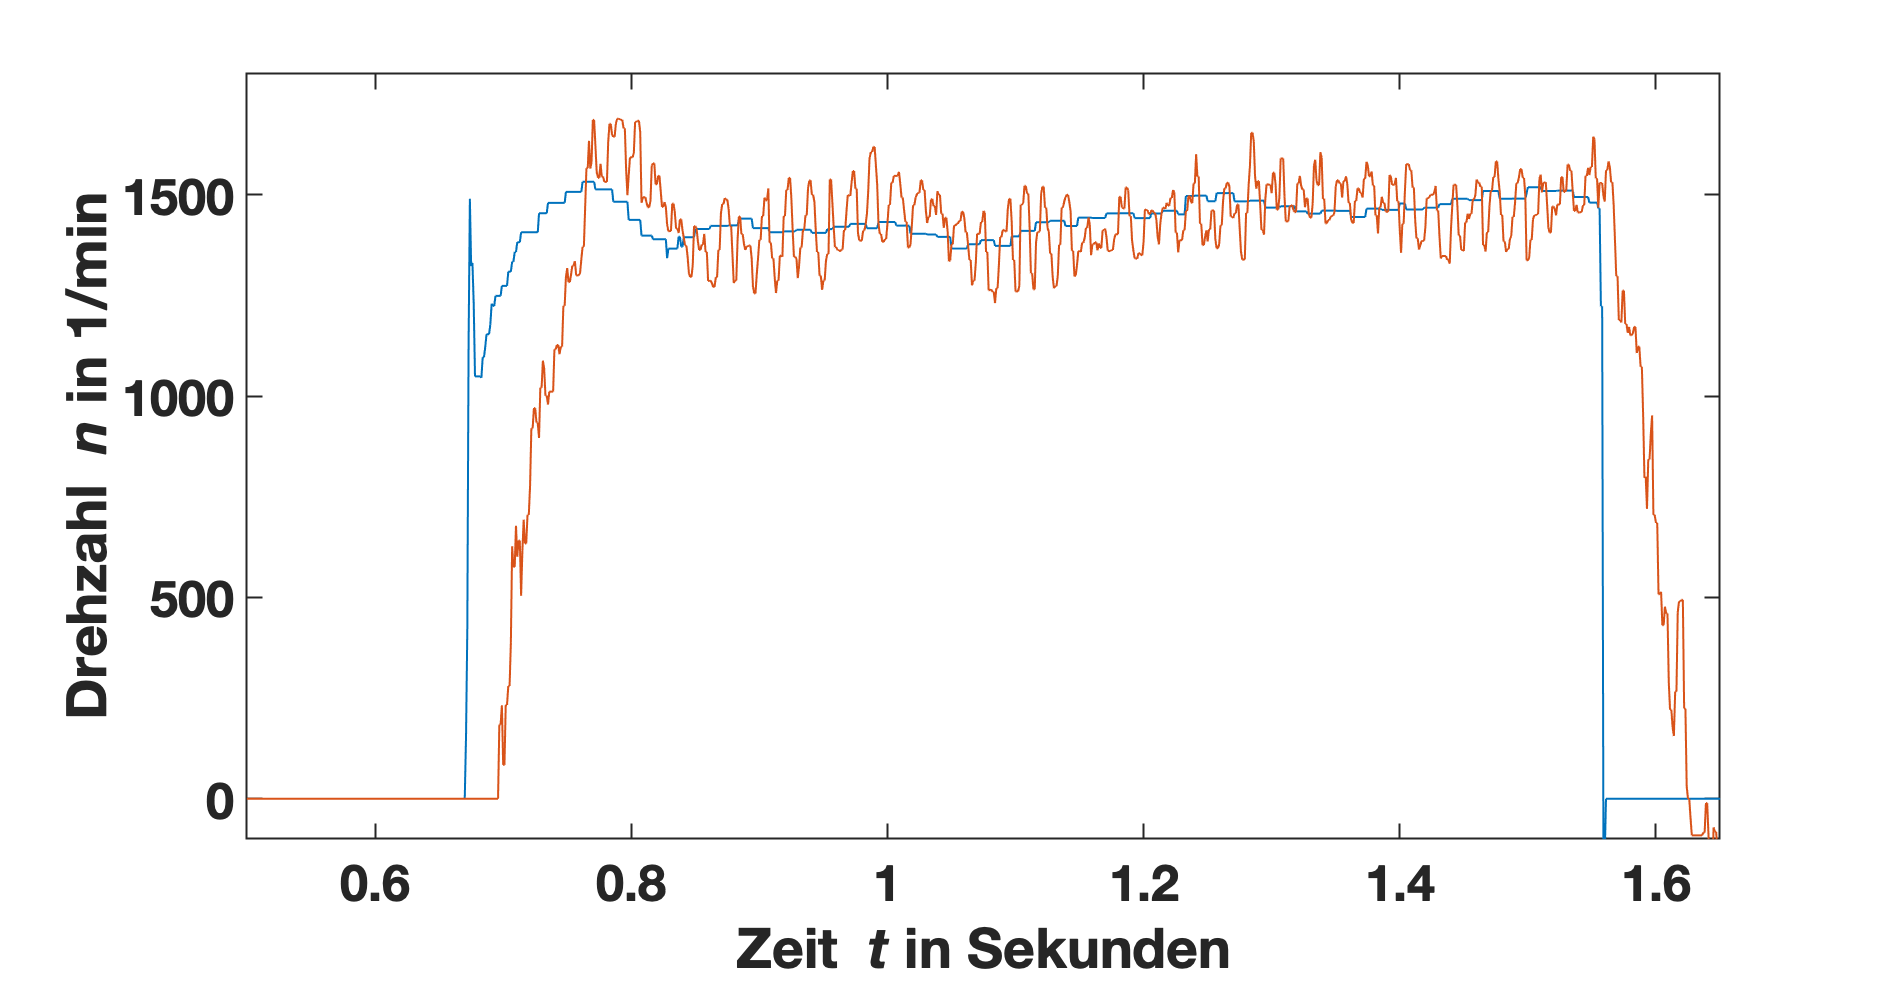
\includegraphics[width=1.0\textwidth]{Bilder/regler_real.png}
					\caption{Regelverlauf am Motor hinten Rechts, mit Sollwert (blau) und Regelgröße (orange)}
					\label{fig: regler_real}
				\end{figure} 

		
		
		\subsection{Winkelregelung}
			\label{subsec: Winkelregelung}
		
		
		Für die Umsetzung der verschiedenen Lenkungsprinzipien aus Kapitel \ref{sec: Unterscheidung der Lenkungsprinzipien} wird für dieses Projekt die Bewegung des Fahrzeugs in zwei Komponenten unterteilt. Der Posenwinkel $\beta$ ist die erste Komponente und beschreibt den Rotationswinkel zwischen dem Koordinatensystem der Karte, in Abbildung \ref{fig: Posen- und Fahrtwinkel} oben rechts dargestellt und der aktuellen Position. Der Fahrtwinkel $\alpha$ stellt die Fahrtrichtung beziehungsweise die Ausrichtung des resultierenden Geschwindigkeitsvektors der Bewegung im Verhältnis zum Odometriekoordinatensystem dar. 
		
		\begin{figure}[H]
			\centering
			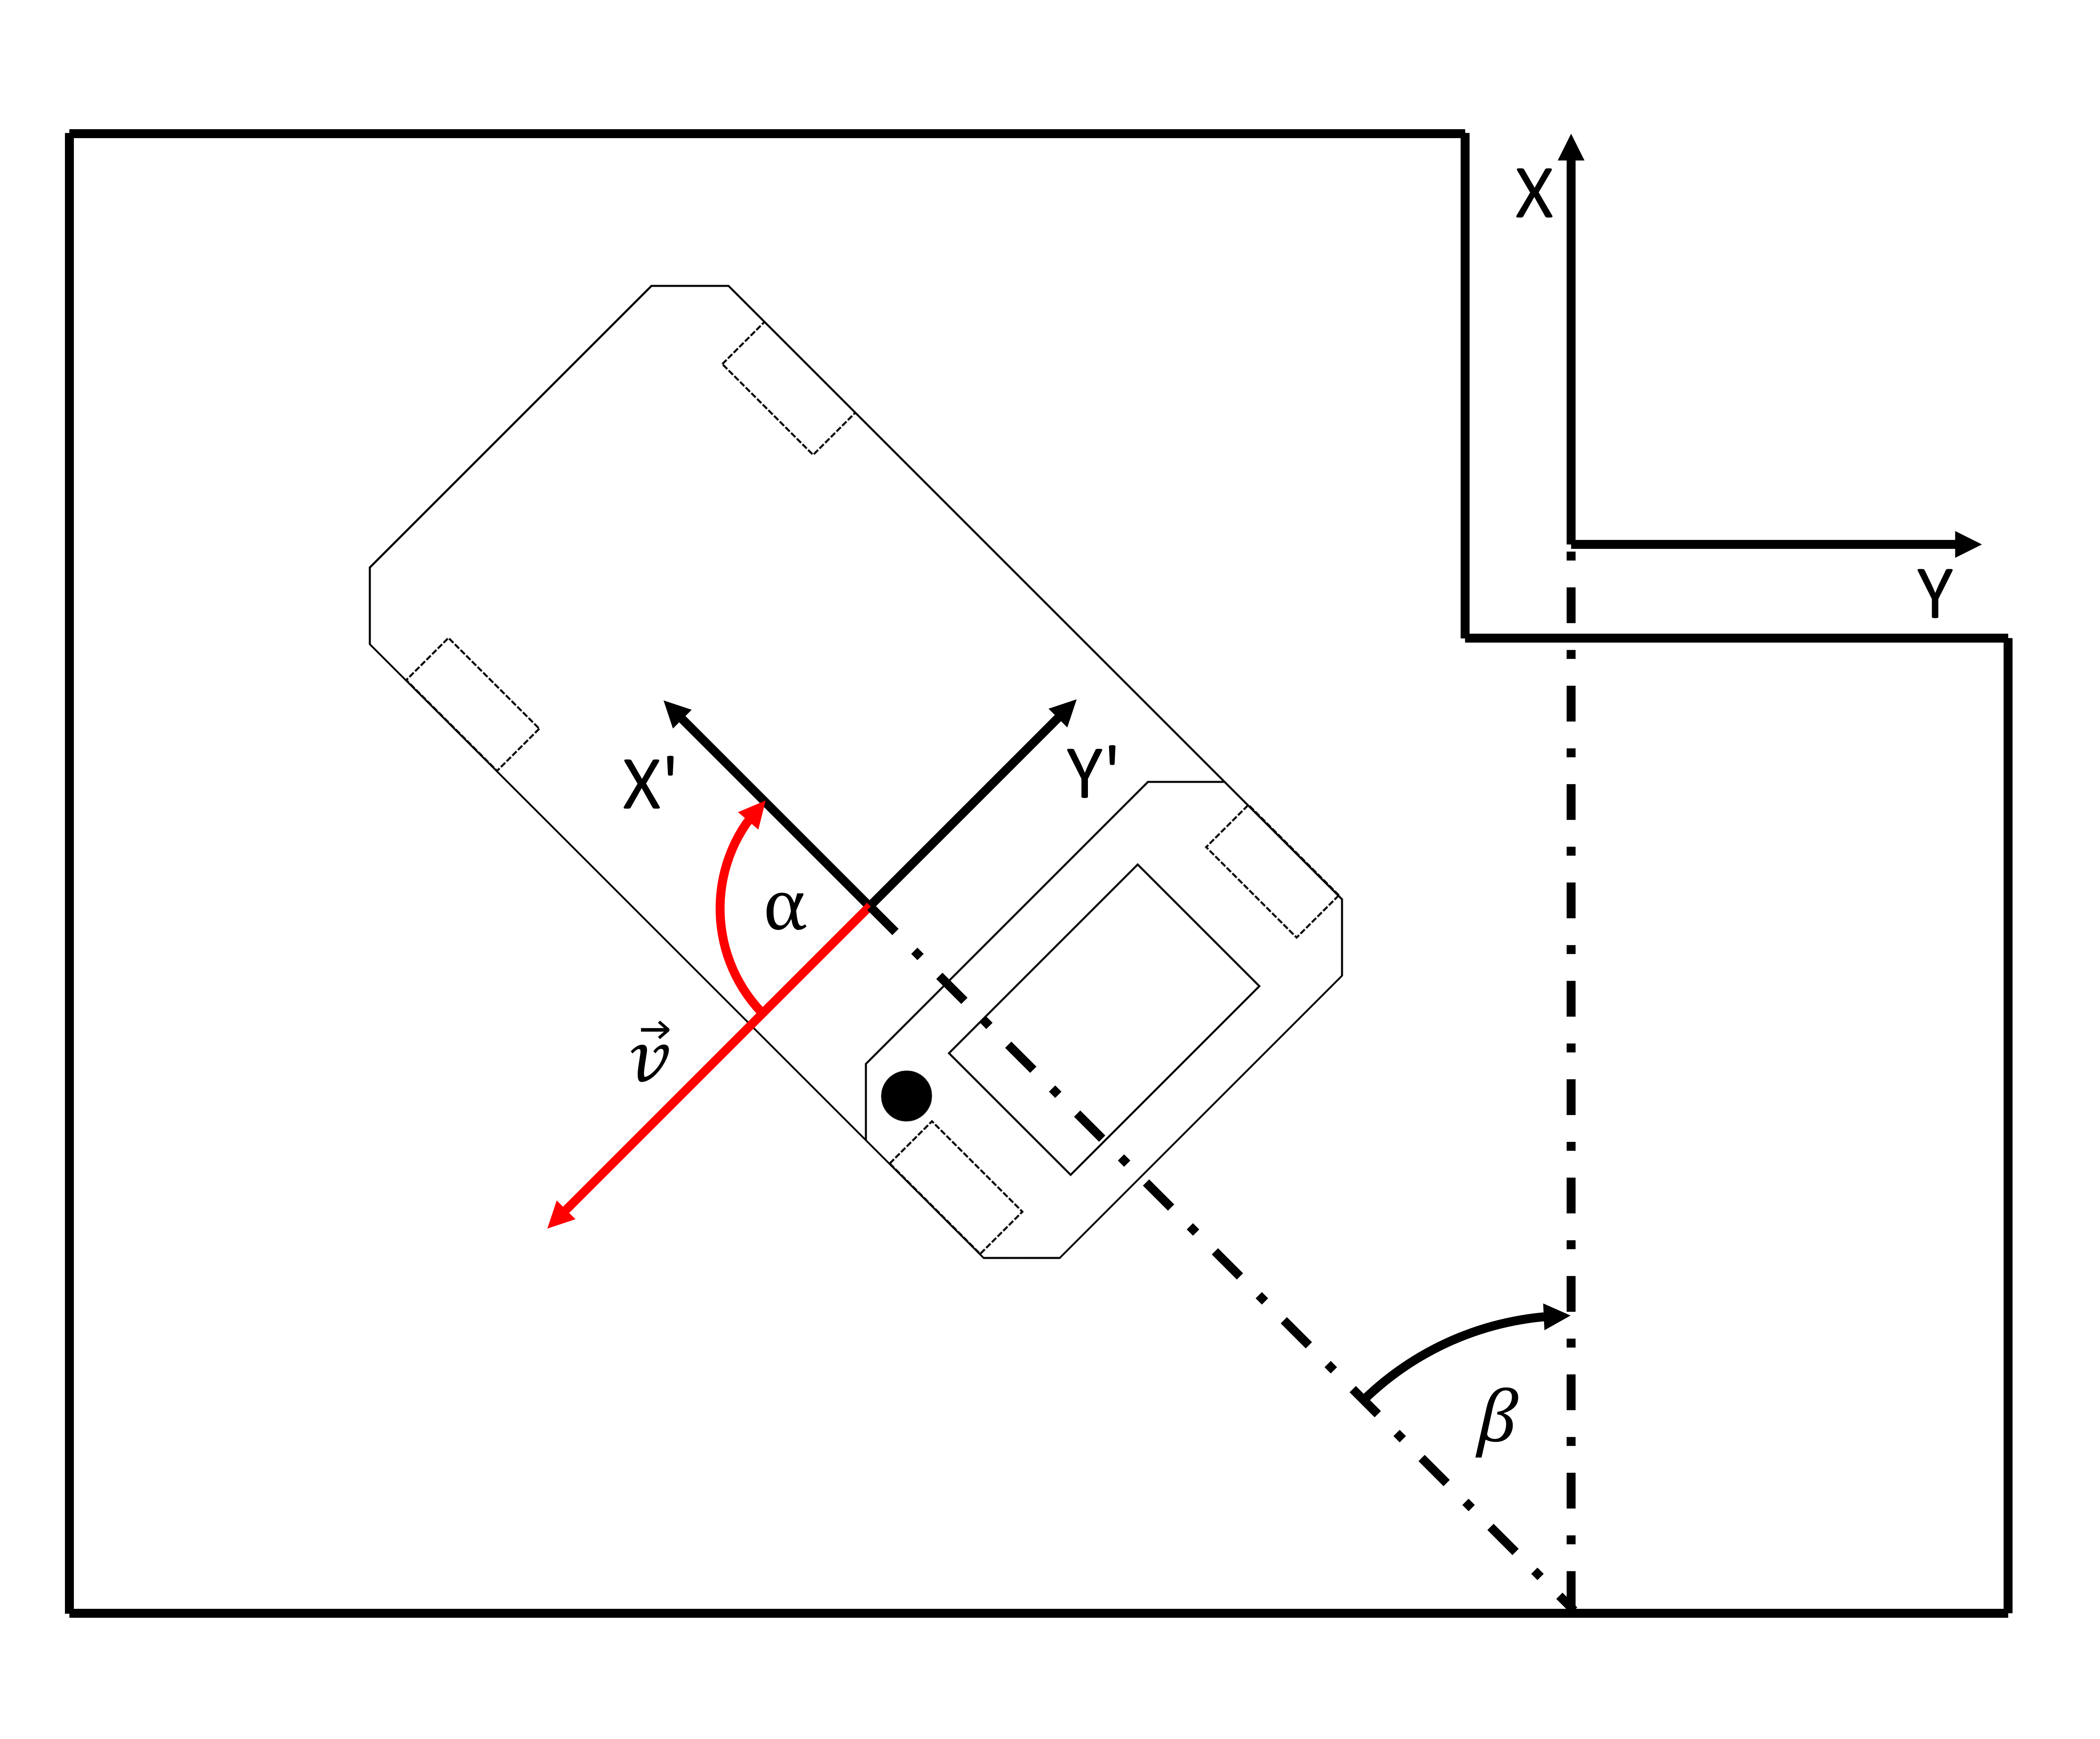
\includegraphics[width=0.8\textwidth]{Bilder/posenundfahrtwinkel.png}
			\caption{Darstellung des Posen- und Fahrtwinkels}
			\label{fig: Posen- und Fahrtwinkel}
		\end{figure}
		
		Mithilfe dieser Unterteilung wird ein translatorisches Bewegungsziel rotatorisches Posenwinkel vorgegeben. Das Prinzip wird durch zwei vierdimensional Vektoren realisiert, wobei jeder Zeileneintrag für jeweils ein Rad als Multiplikator der Drehzahl genutzt wird. Die beiden Ziele können rechnerisch durch eine Addition der Vektoren vereint werden und ergeben ein neues, gemeinsames Bewegungsziel.     
		
		\begin{figure}[H]
			\centering
			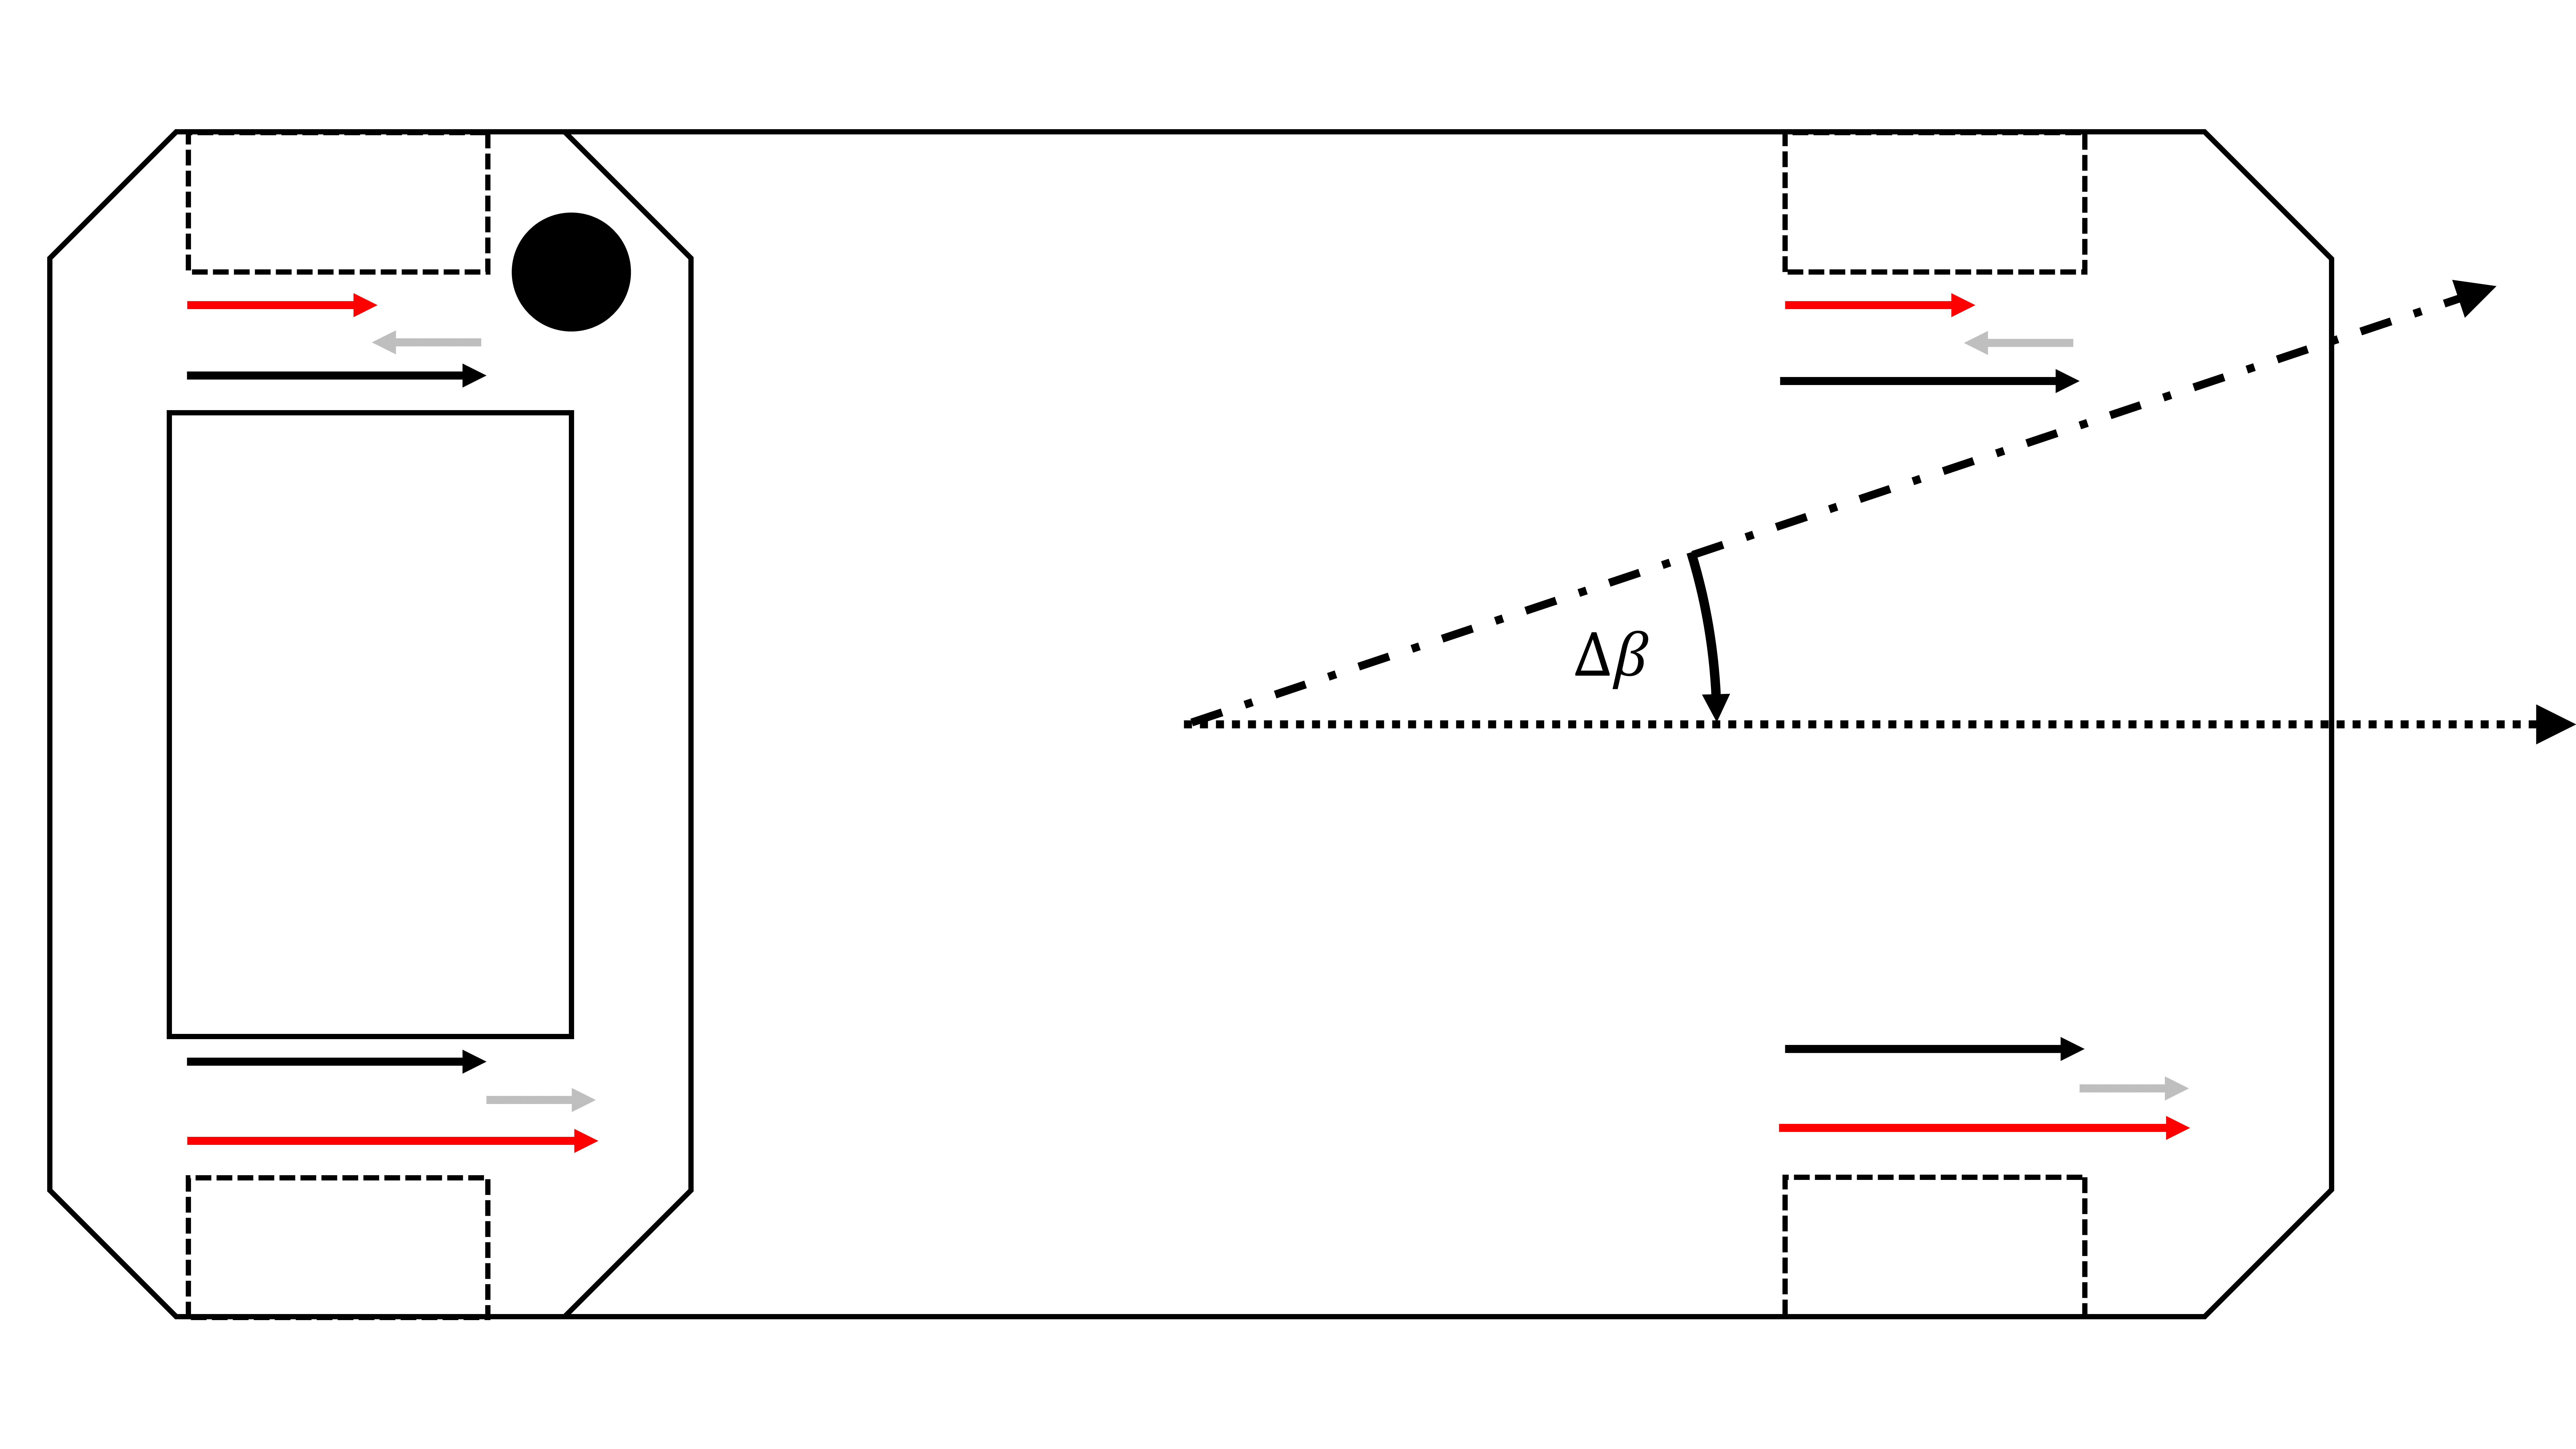
\includegraphics[width=1.0\textwidth]{Bilder/winkelregelung.png}
			\caption{Darstellung des Funktionsprinzips der Winkelregelung}
			\label{fig: Winkelregelung}
		\end{figure}
		
		In Abbildung \ref{fig: Winkelregelung} ist die Funktionsweise der Winkelregelung prinzipiell dargestellt. Das Fahrzeug soll sich hier beispielhaft mit einem Fahrtwinkel von 0$^\circ$ entlang des grünes Pfeils, der als Strichpunktlinie dargestellt ist, ausrichten und geradeaus fahren. Der rote, als Strichpunktlinie dargestellte Pfeil zeigt die momentane Ausrichtung der Pose. Die schwarzen Pfeile sollen den Betrag und die Richtung der Einträge des aus den Fahrtwinkel errechneten Vektors darstellen. Der Posenwinkel muss in diesem Beispiel korrigiert werden und erzeugt ein Vektor der hier mit roten Pfeilen symbolisch gezeigt wird. Nach der oben genannten Addition ergibt sich der resultierende Vektor, der in Abbildung \ref{fig: Winkelregelung} mit grünen Pfeilen beschrieben wird. 
		
		
		
		\begin{align}
		\label{eq: gpi1}
		G_{pi1}(s) &= \frac{0.07403s+0.07793}{0.9499s}\\\nonumber\\
		\label{eq: gpi2}
		G_{pi2}(s) &= \frac{0.0582s+0.04546}{1.14s}\\\nonumber\\
		\label{eq: gpi3}
		G_{pi2}(s) &= \frac{0.1s+0.005}{s}
		\end{align}
		
		\begin{equation}
		\vec{v}=\left(
		\begin{array}{c}
		\frac{b}{\sin(\frac{\omega}{2})}\\
		\frac{c}{\sin(\frac{\omega}{2})}\\
		\frac{d}{\sin(\frac{\omega}{2})}\\
		\end{array}\right) \text { mit }  \omega =2\cdot\arccos(a)
		\label{eq: quaternion vektorlage}
		\end{equation}\newline
		
		\begin{equation}
		\sigma \cdot \vec{a} + \gamma \cdot \vec{a} + \vec{b} \cdot \underline{M} = \vec{g} 
		\label{eq: winkeleq}
		\end{equation}
		
		\begin{equation}
		\sigma = \Delta \beta_{HS} \cdot P_{HS} 
		\end{equation}
			
			
		\begin{equation}
		\gamma = \Delta \beta_{MB} \cdot P_{MB} 
		\end{equation}
		
		\begin{equation}
		\vec{a} = \left(
		\begin{array}{r}
		-1\\
	    1\\
		-1\\
		1\\
		\end{array}\right)
		\end{equation}
			
	\section{Autonomes Fahren}
	\label{sec:Autonomes Fahren}

		\subsection{Auswerten der Sensordaten}
		\label{subsec: Auswerten der Sensordaten}
		
			\subsubsection{Visualisierung der Sensordaten}
			\label{subsubsec: Visualisierung der Sensordaten}
			
			ROS Visualization, oder auch Rviz genannt, ist ein 3D-Visualisierungstool und wird für die Anzeige von Sensordaten und Statusinformationen genutzt. Zur Visualisierung des Robotermodels in Rviz, wird eine Unified Robot Description Format (URDF) Datei erstellt \cite{urdf}. In der URDF Datei werden vom Benutzer dreidimensionale Körper programmiert und ausgerichtet. In Abbildung \ref{fig: URDF} ist das mit der URDF Datei erzeugte und in Rviz visualisierte ALF zu sehen.
			
			\begin{figure}[H]
				\centering
				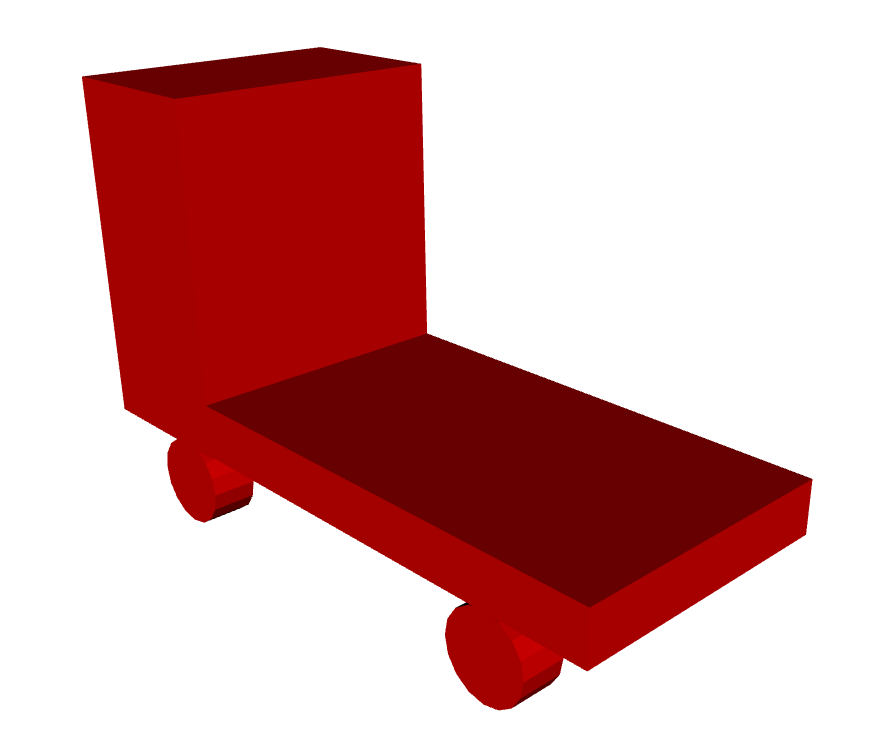
\includegraphics[width=0.6\textwidth]{Bilder/urdf.png}
				\caption{Darstellung des ALFs in Rviz durch eine URDF-Datei}
				\label{fig: URDF}
			\end{figure}
			
			Wenn der Knoten Rviz gestartet wird öffnet sich eine Benutzeroberfläche auf der die entsprechenden Topics abonniert werden können. Für eine bessere Übersicht lassen sich die visualisierten Sensordaten einfärben, um diese später voneinander unterscheiden zu können. Ebenfalls ist es möglich in Rviz eine 2D-Pose einzugeben, die als Navigationsziel für den in Kapitel \ref{subsec: Kartografierung und Bewegungsplanung} erklärten Trajektorie Planer dient. \cite{rviz}  
		
		    \subsubsection{Integration der Laserdaten}
		    \label{subsubsec: Übersetzen der Laserdaten}
		    	
		    	Die Integration der Messwerte des RPLIDAR A2 Sensors in das ROS-Netzwerk wird durch den Knoten \glqq Rplidar\grqq{} umgesetzt. Bei dem Aufruf des Knotens wird der Motor des $360^\circ$-Laserscanners gestartet und die Topic \glqq Scan\grqq{} mit dem Nachrichtentyp \glqq LaserScan \grqq{} veröffentlicht. In Abbildung \ref{fig: Laserscan des RPLIDAR in Rviz} sind Beobachtungen von Landmarken des Lidar Sensors als schwarze Punkte zu sehen. \cite{rplidar}
		    	
		    	\begin{figure}[H]
		    		\centering
		    		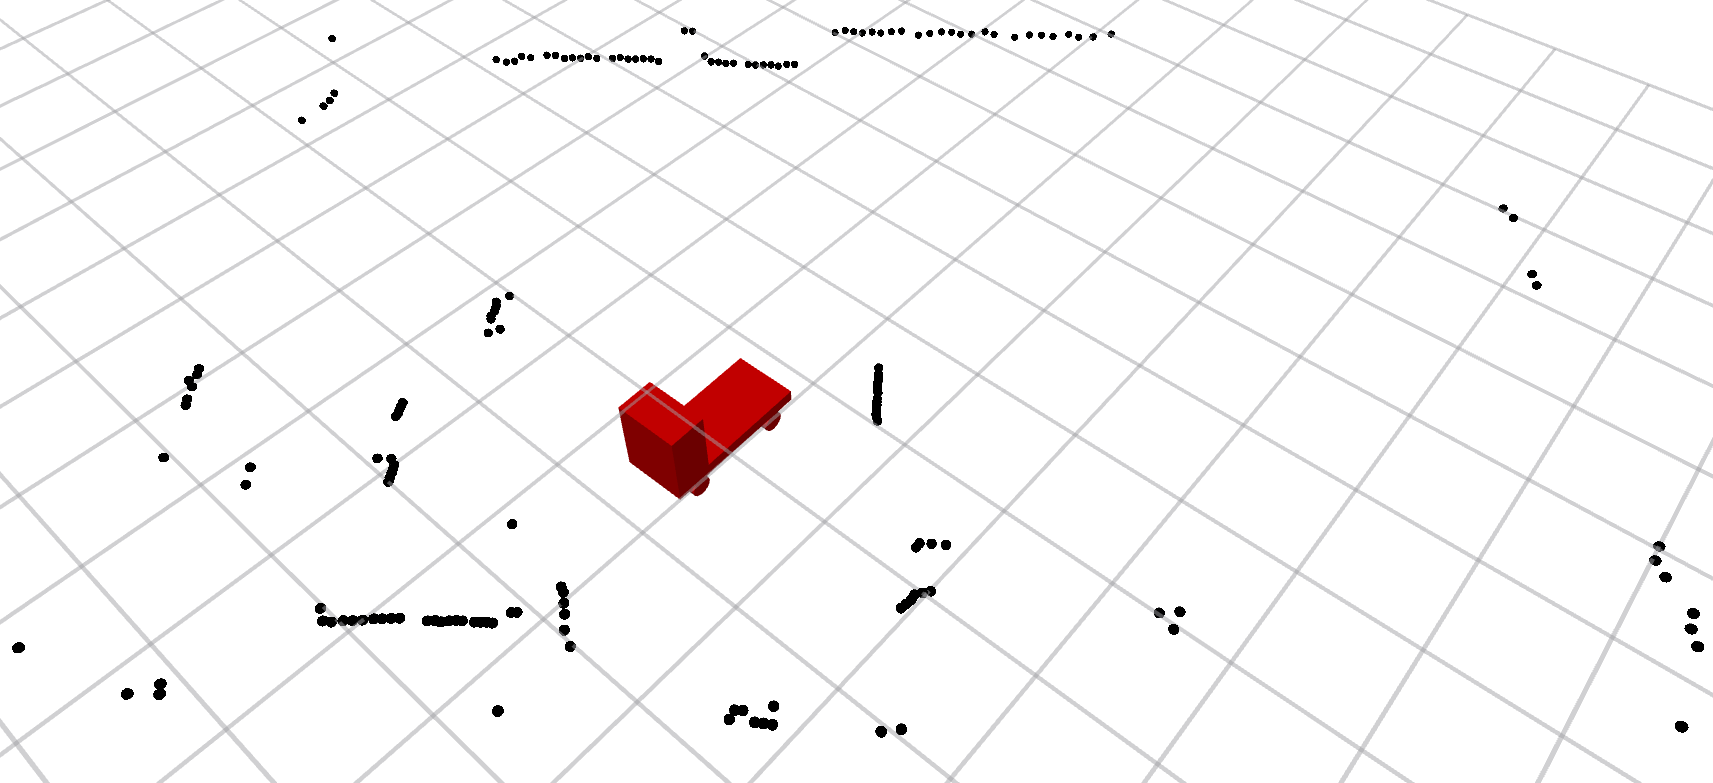
\includegraphics[width=1.0\textwidth]{Bilder/laserscan.png}
		    		\caption{Darstellung der Laserscan-Daten des Lidar-Sensors in Rviz}
		    		\label{fig: Laserscan des RPLIDAR in Rviz}
		    	\end{figure}
		    
		    	
		    \subsubsection{Integration der Kinect-Sensoren}
		    \label{subsubsec: Kinect-Sensor}	    
		    
		    	Für die Implementieren der von den Kinect-Sensoren aufgenommenen Bildinformationen in das ROS-Netzwerk wird in dieser Bachelorarbeit der Knoten \glqq Kinect2 Bridge\grqq{} benutzt. Das Softwarepaket enthält eine Kalibrierung, eine Registrierung, ein eigenständiges Anzeigewerkzeug für das Kamerabild und einige Knoten für die Veröffentlichung aller Kamerafunktionen als Topic. 
		    	
		    	Um Softwareabstürze zu vermeiden, die bei der Inbetriebnahme von zwei Kinect Kameras auftreten, wird der Buffer des Universal Serial Bus Filesystem (USBFS) vergrößert \cite{libfreenect2troubleshooting}.
		    	Zudem wird die Bildrate auf maximal 5 Bilder pro Sekunde reduziert,anschließend konnten beide Kinect-Snsoren ohne Probleme betrieben werden. \cite{iaikinect}\\
		   		    
		    	Die vom Knoten \textit{Kinect2 Bridge} veröffentlichte Topic \textit{kinect2/hd/image\_depth\_rect} ist vom Nachrichtentyp \textit{Image }und kann von dem in Kapitel \ref{subsubsec: Erstellen der Bewegungsplanung} beschriebenen Knoten \textit{Move Base} nicht verwendet werden, weil dieser Nachrichten von dem Typ \textit{LaserScan} benötigt.
			    Deshalb wird der Knoten \textit{Depthimage To Laserscan} benutzt, um eine Typkonvertierung von \textit{Image} zu \textit{ LaserScan} durchzuführen.
		    	Ein relevanter Parameter für die Typkonvertierung ist \textit{scan\_height}, der die genutzte Anzahl der horizontal angelegten Pixelreihen des Bildes beschreibt. Der Knoten verwendet den kleinsten gemessenen Abstand einer Spalte und benutzt diesen Wert für die Nachricht \textit{LaserScan}.
		    	Als Ergebnis der Typkonvertierung können die Kinect-Sensoren für die Navigation als Observierungsquelle genutzt werden.
		    	 Im Rahmen dieser Bachelorarbeit werden die konvertierten Nachrichten des Typs \textit{LaserScan} in den Topics \textit{Scan1} und \textit{Scan2} von den beiden Kinect-Sensoren veröffentlicht. \cite{depthimagetolaserscan}
		    	
		   
		     	\begin{figure}[H]
		     		\centering
		     		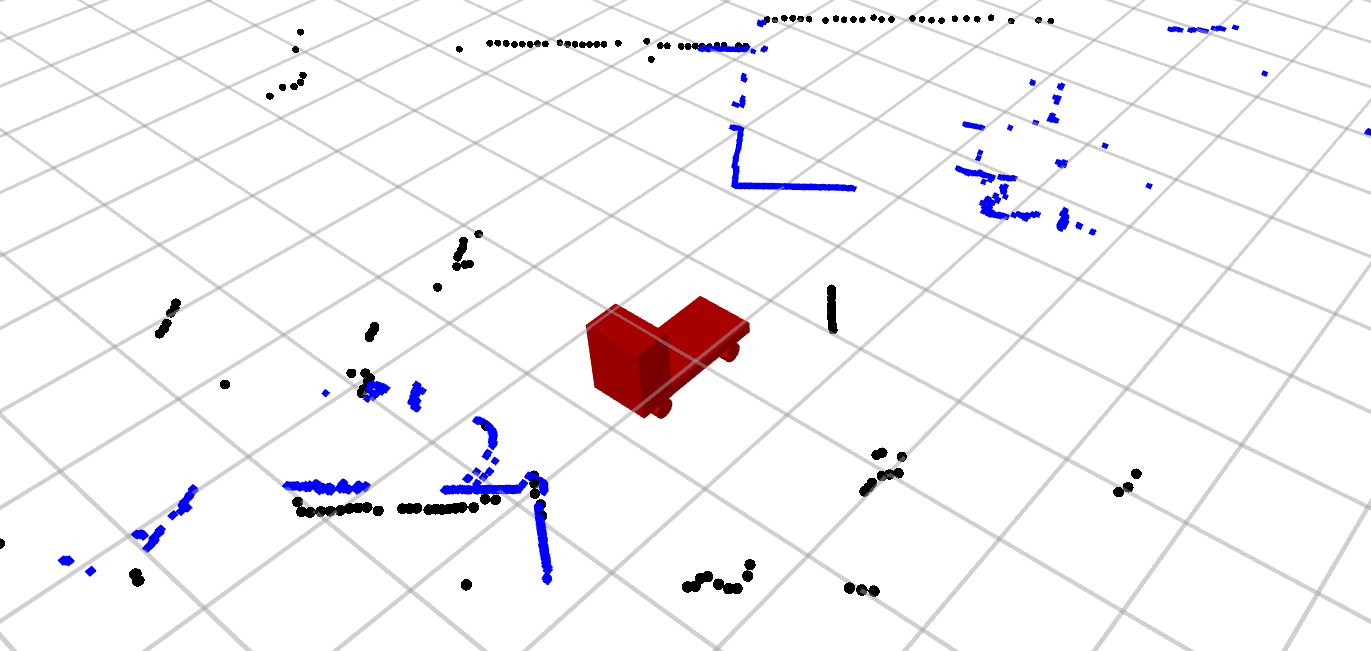
\includegraphics[width=1.0\textwidth]{Bilder/lidarundkinect.png}
		     		\caption{Darstellung der Laserscan-Daten in Rviz}
		     		\label{fig: Laserscans in Rviz}
		     	\end{figure}
		     	
		     	In Abbildung \ref{fig: Laserscans in Rviz} sind die Laserscan-Daten des Lidar-Sensors als schwarze und der beiden Kinect-Sensoren als blaue Punkte dargestellt. Oben rechts und unten links in der Abbildung ist zu erkennen, dass die Sensordaten teilweise nicht korrelieren. Dies ist auf die Kinect-Sensoren zurückzuführen, weil Objekte unter der Arbeitshöhe des 360$^\circ$-Laserscanners liegen erkannt werden. In der Abbildung \ref{fig: Verifikation der erfassten Laserdaten} können die in Abbildung \ref{fig: Laserscans in Rviz} gezeigten Laserdaten nachvollzogen und realen Objekten zugeordnet werden.
		     	
		     %	Dies bedeutet nicht, dass fehlerhafte Daten vorliegen oder die Koordinatentransformation falsch durchgeführt wurde sondern dass Objekte, die unter die Arbeitshöhe des 360$^\circ$-Laserscanners fallen von den Kinect-Sensoren erfasst werden.
		     	
		     	\begin{figure}[H]
		     		\centering
		     		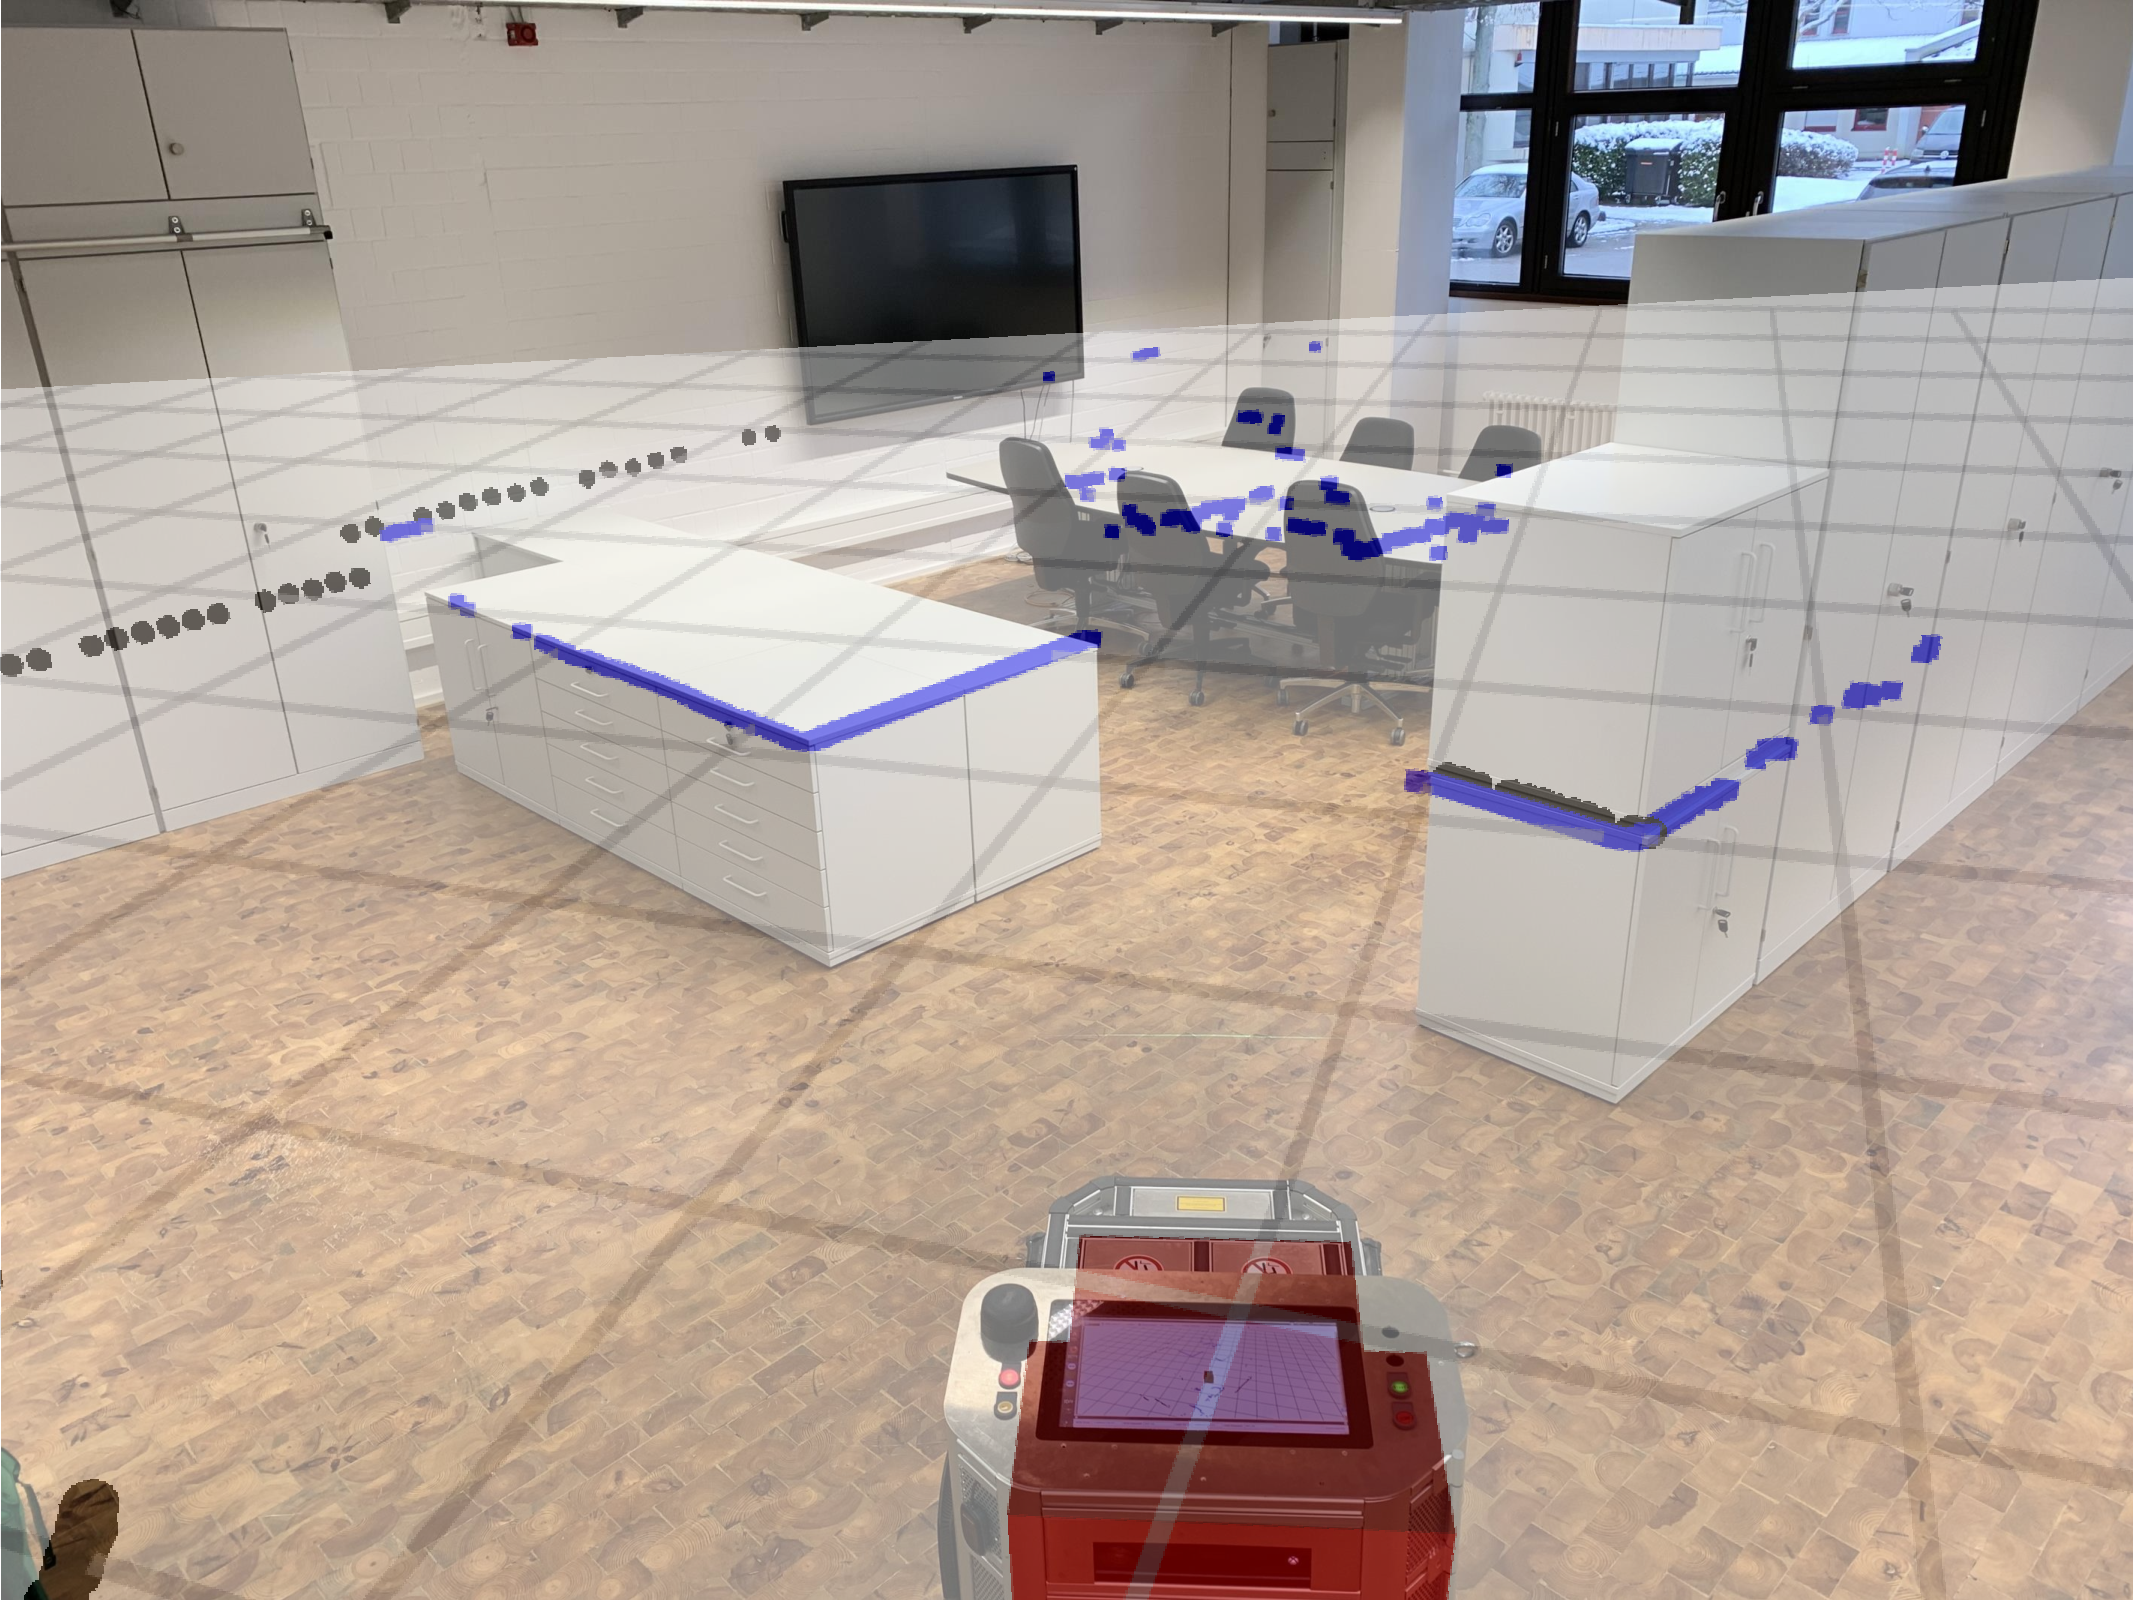
\includegraphics[width=1.0\textwidth]{Bilder/match.pdf}
		     		\caption{Visualisierung der LaserScan Topics aus den Kapiteln \ref{subsubsec: Übersetzen der Laserdaten} und \ref{subsubsec: Depthimage to laserscan} in Rviz. Zum Vergleich ist ein Foto aus gleicher Perspektive unter das Bildschirmfoto aus Rviz gelegt. Die erfassten Gegenstände der Kinect-Sensoren sind in diesem Fall als blaue Markierungen und die des RPLIDAR A2 als schwarz dargestellt. Die Kinect-Sensoren erkennen im Zentrum der Darstellung einen Schrank, der von dem RPLIDAR A2 Sensor nicht erfasst wird. In Kapitel \ref{subsubsection: Hector Mapping} wird genauer auf die Folgen dieser Beobachtung eingegangen.}
		     		\label{fig: Verifikation der erfassten Laserdaten}
		     	\end{figure}
		     	
		     \subsubsection{Anbindung der Fernsteuerung}
		     \label{subsubsec: Anbindung des Xbox-Controllers}
		     
		     \begin{figure}[H]
		     	\centering
		     	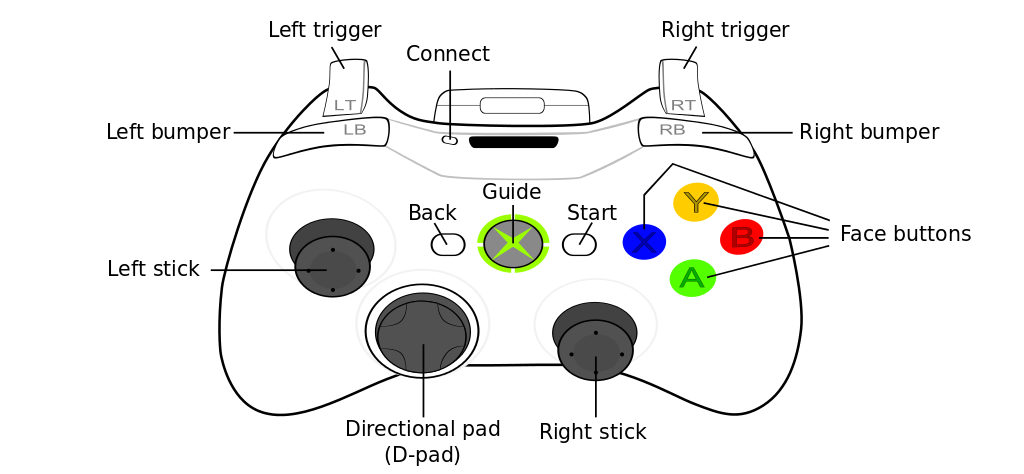
\includegraphics[width=0.8\textwidth]{Bilder/xboxcontroller.png}
		     	\caption{Layout des XBox 360 Controllers}
		     	\label{fig: Layout des XBox 360 Controllers}
		     \end{figure} 
		     
		     	Der Knoten Joy ist für die Konvertierung der vom Benutzer eingegebenen, mechanischen Signale am Joystick zu nutzbaren digitalen Signalen zuständig. Die Betätigung der Knöpfe, wie beispielsweise den farblichen auf der rechten Seite des in Abbildung \ref{fig:  Layout des XBox 360 Controllers} gezeigten Controllers, wird in ein binären Signal umgewandelt. Bei den Joysticks und Triggern werden je nach Lage Zahlenwerte zwischen -1 und 1 in die Topic Joy veröffentlicht. \cite{joy}
		     
		\subsection{Kartografierung und Bewegungsplanung}
		    \label{subsec: Kartografierung und Bewegungsplanung}
		        
		        Das Lastenheft \ref{it: Lastenheft} sieht vor die Umgebung des ALFs mit und ohne eine Bewegungsvorgabe des Benutzers zu kartographieren. In diesem Kapitel werden die für die Umsetzung nötigen Schritte dargelegt.\\
		    	
		    	Zur Kartographierung der Umgebung wird in dieser Bachelorarbeit der Knoten \textit{Hector Slam} verwendet.
		   		Dieser abonniert standardmäßig die in den Kapitel \ref{subsubsec: Übersetzen der Laserdaten} beschriebene \textit{LaserScan }Nachrichten aus der Topic \textit{Scan} und veröffentlicht eine Karte in das Topic \textit{Map} vom Nachrichtentyp \textit{OccupanyGrid}. Diese kann in \textit{Rviz}, wie in Abbildung \ref{fig: Hector}, visualisiert oder als Bilddatei exportiert werden. Die Karte erweitert sich durch Bewegungen des ALFs. Der Knoten löst die SLAM Problematik aus Abschnitt \ref{subsec: Mathematische Beschreibung des SLAM Problems} mit den Umgebungsdaten des \textit{RPLIDAR A2} ohne Odometrieinformationen zu benötigen. \cite{hectorslam}\\
		   				   		
		   		Die hier verwendeten Observationsquellen erfassen unterschiedliche Messwerte. Dies ist nicht auf eine fehlerhafte Messung zurückzuführen sondern auf den in Kapitel \ref{sec: Sensoren zur Erkennung der Umgebung} beschriebenen Arbeitsbereich. Das Veröffentlichen von mehreren Observationsquellen in eine Topic führt unter diesen Umständen zu Komplikationen mit dem verwendeten Algorithmus.
		   		
		   		
		   		\begin{figure}[H]
		   			\centering
		   			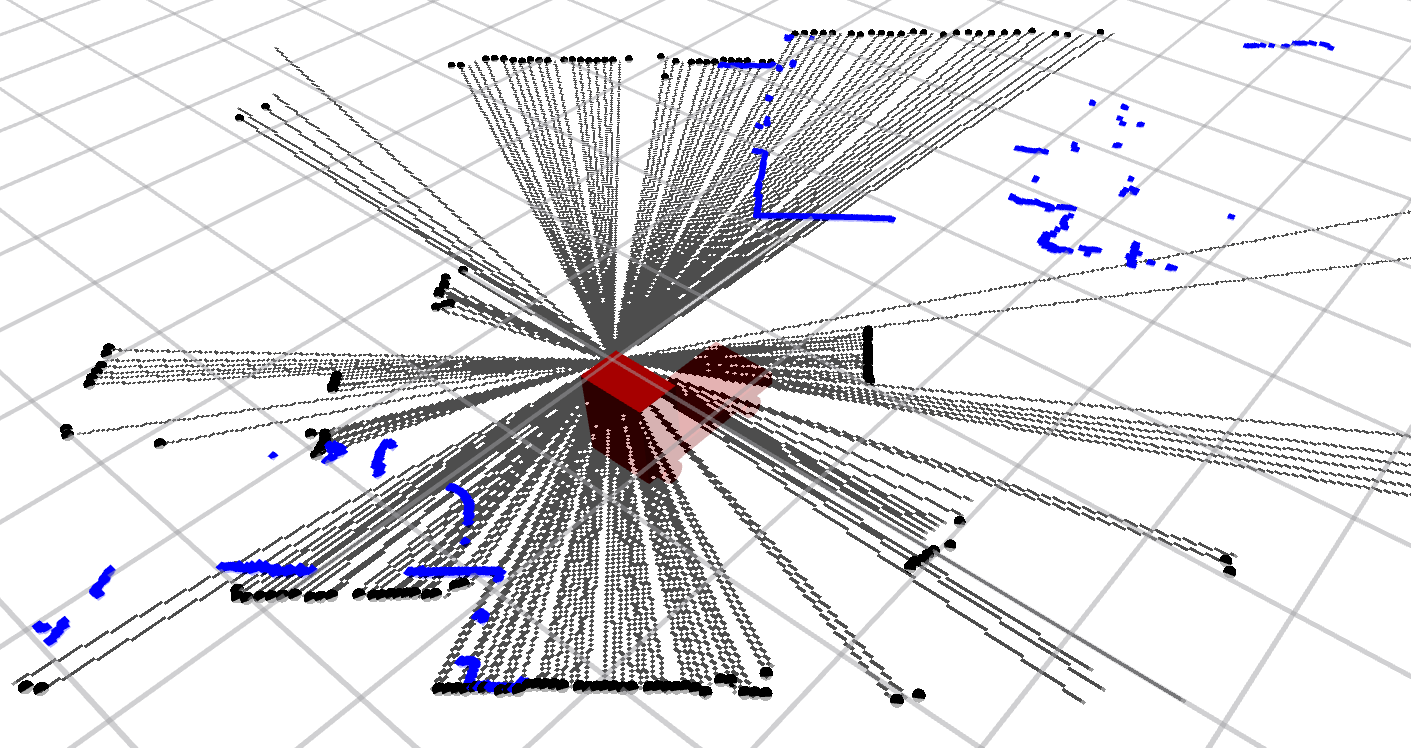
\includegraphics[width=1.0\textwidth]{Bilder/hector}
		   			\caption{Abbildung einer in Rviz dargestellten \textit{OccupancyGrid} Karte aus der Topic \textit{Map} und die \textit{LaserScan} Nachrichten aus Kapitel \ref{subsubsec: Depthimage to laserscan}. Zu sehen ist der Kartographierungsprozess aus der Vogelperspektive. Die schwarzen Punkte repräsentieren \textit{LaserScan} Daten des \textit{RPLIDAR A2} und die blauen der Kinect-Sensoren. Die grauen Linien enden an einer als belegt markierten Zelle und stellen die Karte dar, die sich bei Bewegung des ALFs vervollständigt. Für die Kartographierung in der Abbildung wurden lediglich Messwerte des \textit{RPLIDAR A2} genutzt. }
		   			\label{fig: Hector}
		   		\end{figure}
		   		
		   		Desweiteren veröffentlicht der Knoten die Topic \glqq slam out pose\grqq{} des Nachrichtentyps \glqq Pose \grqq{} mit einer Schätzung der aktuellen Roboterposition. In diesem Nachrichtentyp wird die Orientierung des Roboters durch ein Quaternion beschrieben. Für die Verwendung des Knotens \textit{Hector Slam} ist es notwendig einen Baum aus statischen Koordinatentransformationen zu erstellen, der die Positionen aller Sensoren relativ zur geschätzten Roboterpose enthält. \cite{hectorslam}
		   		
		   		\begin{figure}[H]
		   			\centering
		   			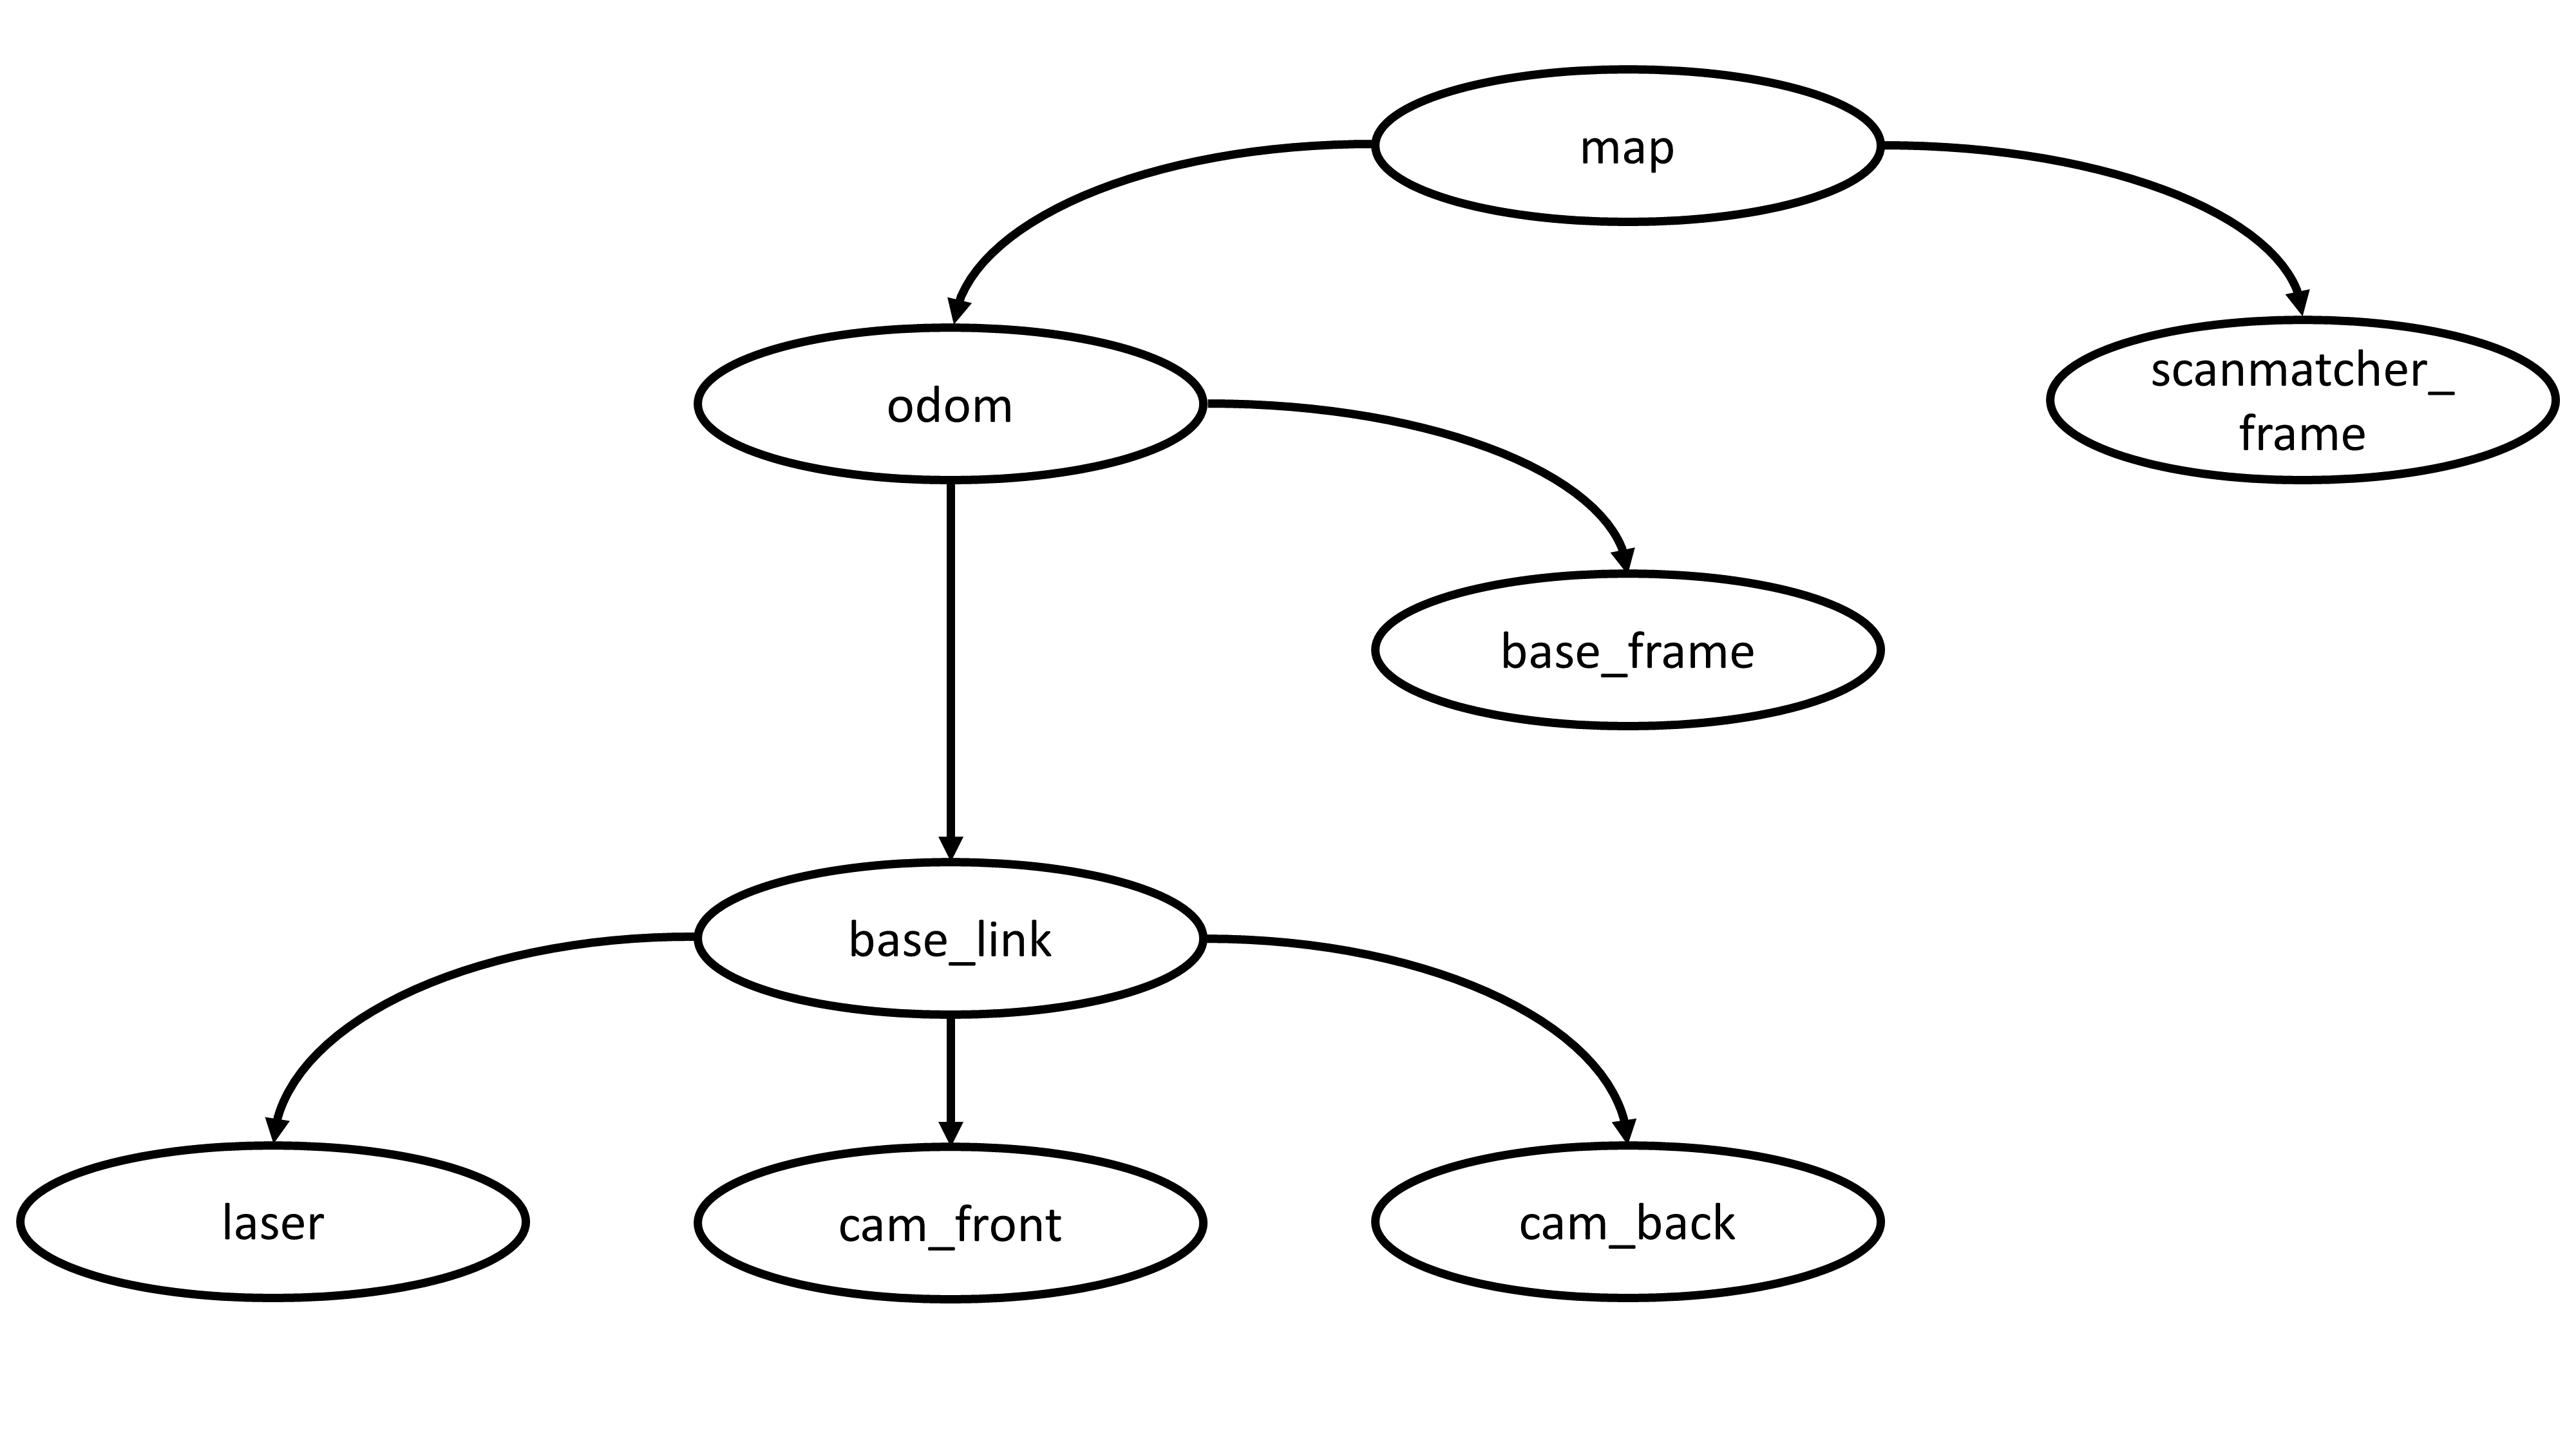
\includegraphics[width=1.0\textwidth]{Bilder/frames}
		   			\caption{Darstellung der Baumstruktur der in diesem Projekt verwendeten Koordinatentransformationen}
		   			\label{fig: Baum der Koordinatentransformationen}
		   		\end{figure}
		      		    
		        Die in Abbildung \ref{fig: Baum der Koordinatentransformationen} dargestellten, dynamischen Transformationen map $\rightarrow$ odom und map $\rightarrow$ scanmatcher\_frame werden von \textit{Hector Mapping} durchgeführt. Der \textit{Static Transform Publisher} veröffentlicht statische Koordinatentransformationen in das Topic \textit{tf}. \cite{sttrpu}
		 			    
		 			    
		    \subsubsection*{Erstellen der Bewegungsplanung}
		    \label{subsubsec: Erstellen der Bewegungsplanung}
		    
		    	Das Softwarepaket \textit{Navigation} enthält Anwendungen um eine Zielpose in Geschwindigkeitsbefehle umzuwandeln und in einer Topic zu veröffentlichen. Die Hauptanwendung des Pakets ist der Knoten \textit{Move Base}. Dieser abonniert Observationsquellen, eine OccupancyGrid Karte, Koordinatentransformationen oder Odometrieinformationen und 2D-Zielposen aus dem ROS-Netzwerk. Der Knoten veröffentlicht ein Bewegungsziel und Costmaps, die in Abschnitt xy erläutert werden. \cite{navigation,movebase}\\ 
		    	
		    	In dieser Bachelorarbeit werden die Topics \textit{Scan}, \textit{Scan1} und \textit{Scan2} von den in Kapitel \ref{subsubsec: Übersetzen der Laserdaten} und \ref{subsubsec: Kinect-Sensor} beschriebenen Observierungsquellen abonniert. Des Weiteren werden die Informationen über Koordinatentransformationen und 2D-Zielposen aus den Topics \textit{tf} sowie \textit{/move\_base\_simple/goal} abonniert. 
		    	
		    	Der Knoten \textit{Move Base }ist in einzelnen Teilanwendungen aufgeteilt. Der enthaltene Global Planner wandelt eine Zielpose in eine Trajektorie um. Durch einen externen Knoten, wie zum Beispiel Rviz, kann ein solches Ziel im ROS-Netzwerk veröffentlicht werden.
		    	 Aus der Trajektorie des \textit{Global Planners} und der geschätzten Position des Roboters erstellt der \textit{Local Planner} das Topic \textit{cmd\_vel}. Dieses beinhaltet eine Bewegungsplanung, resultierend aus der aktuellen Positionsschätzung und der geplanten Trajektorie. In dieser Bachelorarbeit dient das Topic als Grundlage für die Erstellung des Bewegungsziels aus Kapitel \ref{subsec: Winkelregelung}. \cite{movebase,cmdvel}\\
		    	
		    	Der in diesem Projekt verwendete Teb Local Planner gilt als Plugin für den in Move Base vorhandenen Local Planner und arbeitet nach der Timed Elastic Band Methode (TEB). Durch eine prädiktive Regelung, die durch die TEB-Methode beschrieben ist, lassen sich Vorhersagen über die abzufahrende Trajektorie tätigen, die kontinuierlich optimiert wird. \cite{tebmethode} \\
		    	
		    	Der Teb Local Planner plant die Trajektorie in Abhängigkeit von dem Roboterumriss aus Abbildung \ref{fig: footprint} und der zugrunde liegenden Costmap, welche im folgenden erkärt wird. \cite{tebmethode}.
		    	
		    	
		    \begin{figure}[H]
		    	\centering
		    	\includegraphics[width=0.8\textwidth]{Bilder/footprint.png}
		    	\caption{Darstellung des Robterumrisses des Fahrzeugs ALF in rot und der daraus resultierenden Radien für die Inflations Schicht. Der Kreismittelpunkt entspricht dem Ursprung des Base Frame Koordinatensystems, welches in Kapitel \ref{subsubsection: Umrechnung der Koordinatensysteme} durch den static transform publisher eingeführt wurde}
		    	\label{fig: footprint}
		  	  \end{figure}
		    
		     Der Roboterumriss ist als Parameter in den entsprechenden Knoten hinterlegt und wird beim Aufruf von Rviz sichtbar. Abbildung \ref{fig: footprint} stellt den Roboterumriss des ALF's dar und beinhaltet die Radien $R_{i}$ und $R_{c}$ , welche als \glqq Inscribed Radius\grqq{} und \glqq Circumscribed Radius\grqq{} bezeichnet werden und für die Erstellung der Costmap von Bedeutung sind \cite{costmap}. Das Softwarepaket abonniert, wie in Kapitel \ref{subsec: Auswerten der Sensordaten} erörtert, die Sensordaten aus der Umgebung und verarbeitet diese zu einer sogenannten Costmap, welche dazu dient die Zellen in Kapitel \ref{subsec: Graph-basierende Techniken} erwähnten Occupancy Grid Karte mit Werten (Costs) zwischen 0 und 254 zu gewichten.
		  	Die entstandene Occupancy Grid Karte besteht aus mehreren Schichten, welche unter anderem Daten über Gegenstände in der Hindernisschicht, Sicherheitsradien in der Inflationsschicht und bereits vorhandenen Karten in der statischen Schicht enthält. In der statischen Schicht wird die oben genannte Occupancy Grid Karte hinterlegt, welche als Basis für die Costmap und deren Werteverteilung dient. In diesem Projekt abonniert die statische Schicht die Topic \glqq Map\grqq{} des in Kapitel \ref{subsubsection: Hector Mapping} beschriebenen Knotens Hector Mapping und bildet somit die Grundlage der Costmap. \cite{costmap}\\
		  	
		  	Die Hindernisschicht abonniert die verarbeiteten Daten aus Kapitel \ref{subsubsec: Übersetzen der Laserdaten} und \ref{subsubsec: Depthimage to laserscan}. Dadurch werden bei Anwesenheit von Hindernissen die entsprechenden Zellen der Occupancy Grid Karte besetzt und mit den Wert 254 belegt. \cite{costmap}\\
		  	
		  	Die Inflationsschicht veröffentlicht Informationen über die Gewichtung umliegender Zellen eines eingetragenen Hindernisses auf Basis des Roboterumrisses und den Radien $R_{i}$ und $R_{c}$. 
		  	Die Gewichtung sinkt mit steigendem Abstand zum Inscribed Radius in Form einer $e$-Funktion und wird mit Gleichung \ref{eq: cost} berechnet. Der Funktionsverlauf kann von einem Anwender in einer Launchfile durch den Roboertumriss, die ROS-Parameter \glqq cost scaling faktor\grqq{} und \glqq inflation radius\grqq{} beeinflusst werden.
		  	In der Gleichung \ref{eq: cost} ist die Distanz zur besetzten Zelle mit $r$ der cost scaling faktor der $e$-Funktion mit $f$ und der Inscribed Radius als $R_{i}$ definiert. \cite{costmap,inflation}
		  		
		  		\begin{equation}
		  		cost(r)=e^{-\cdot f \cdot (r - R_{i})} \cdot 253
		  		\label{eq: cost}
		  		\end{equation}\newline
		  		Die drei Radien haben folgende Bedeutung:
		  		
		  		\begin{itemize}
		  			\item Inscribed Radius: Steht das Zentrum des Roboters auf einer Zelle der Occupancy Grid Karte, deren Entfernung zu einem Hindernis den Betrag des Inscibed Radius oder weniger entspricht, so gäbe es definitiv eine Kollision mit dem eingetragenen Gegenstand unabhängig von der Orientierung des Roboters.\\
		  			
		  			\item Circumscribed Radius: Ähnlich dem inscribed Radius, jedoch ist eine Kollision mit dem Gegenstand abhängig von der Orientierung des Roboters. \\
		  			
		  			\item Inflation Radius: Die Entfernung zum Gegenstand, mit der die Werteverteilung aus Gleichung endet. Die Entfernung zum Gegenstand vom Circumscribed Radius bis zum Infaltion Radius dient als Puffer Zone. Steht das Roboter Zentrum in dieser Zone, so kollidiert der Roboter definitiv nicht mit dem in der Occupancy Grid Karte eingetragenen Gegenstand.
		  		\end{itemize}
		  			    	
		    
		    	Eine Funktionsauswertung und Auftragen der Werte über r mit dem Radius $R_{i}=0.36$ aus Abbildung \ref{fig: footprint} und einen Faktor $f=10$ ergibt den Funktionsverlauf aus Abbildung \ref{fig: costverteilung}.
		    	
		   
		    	 \begin{figure}[H]
		    		\centering
		    		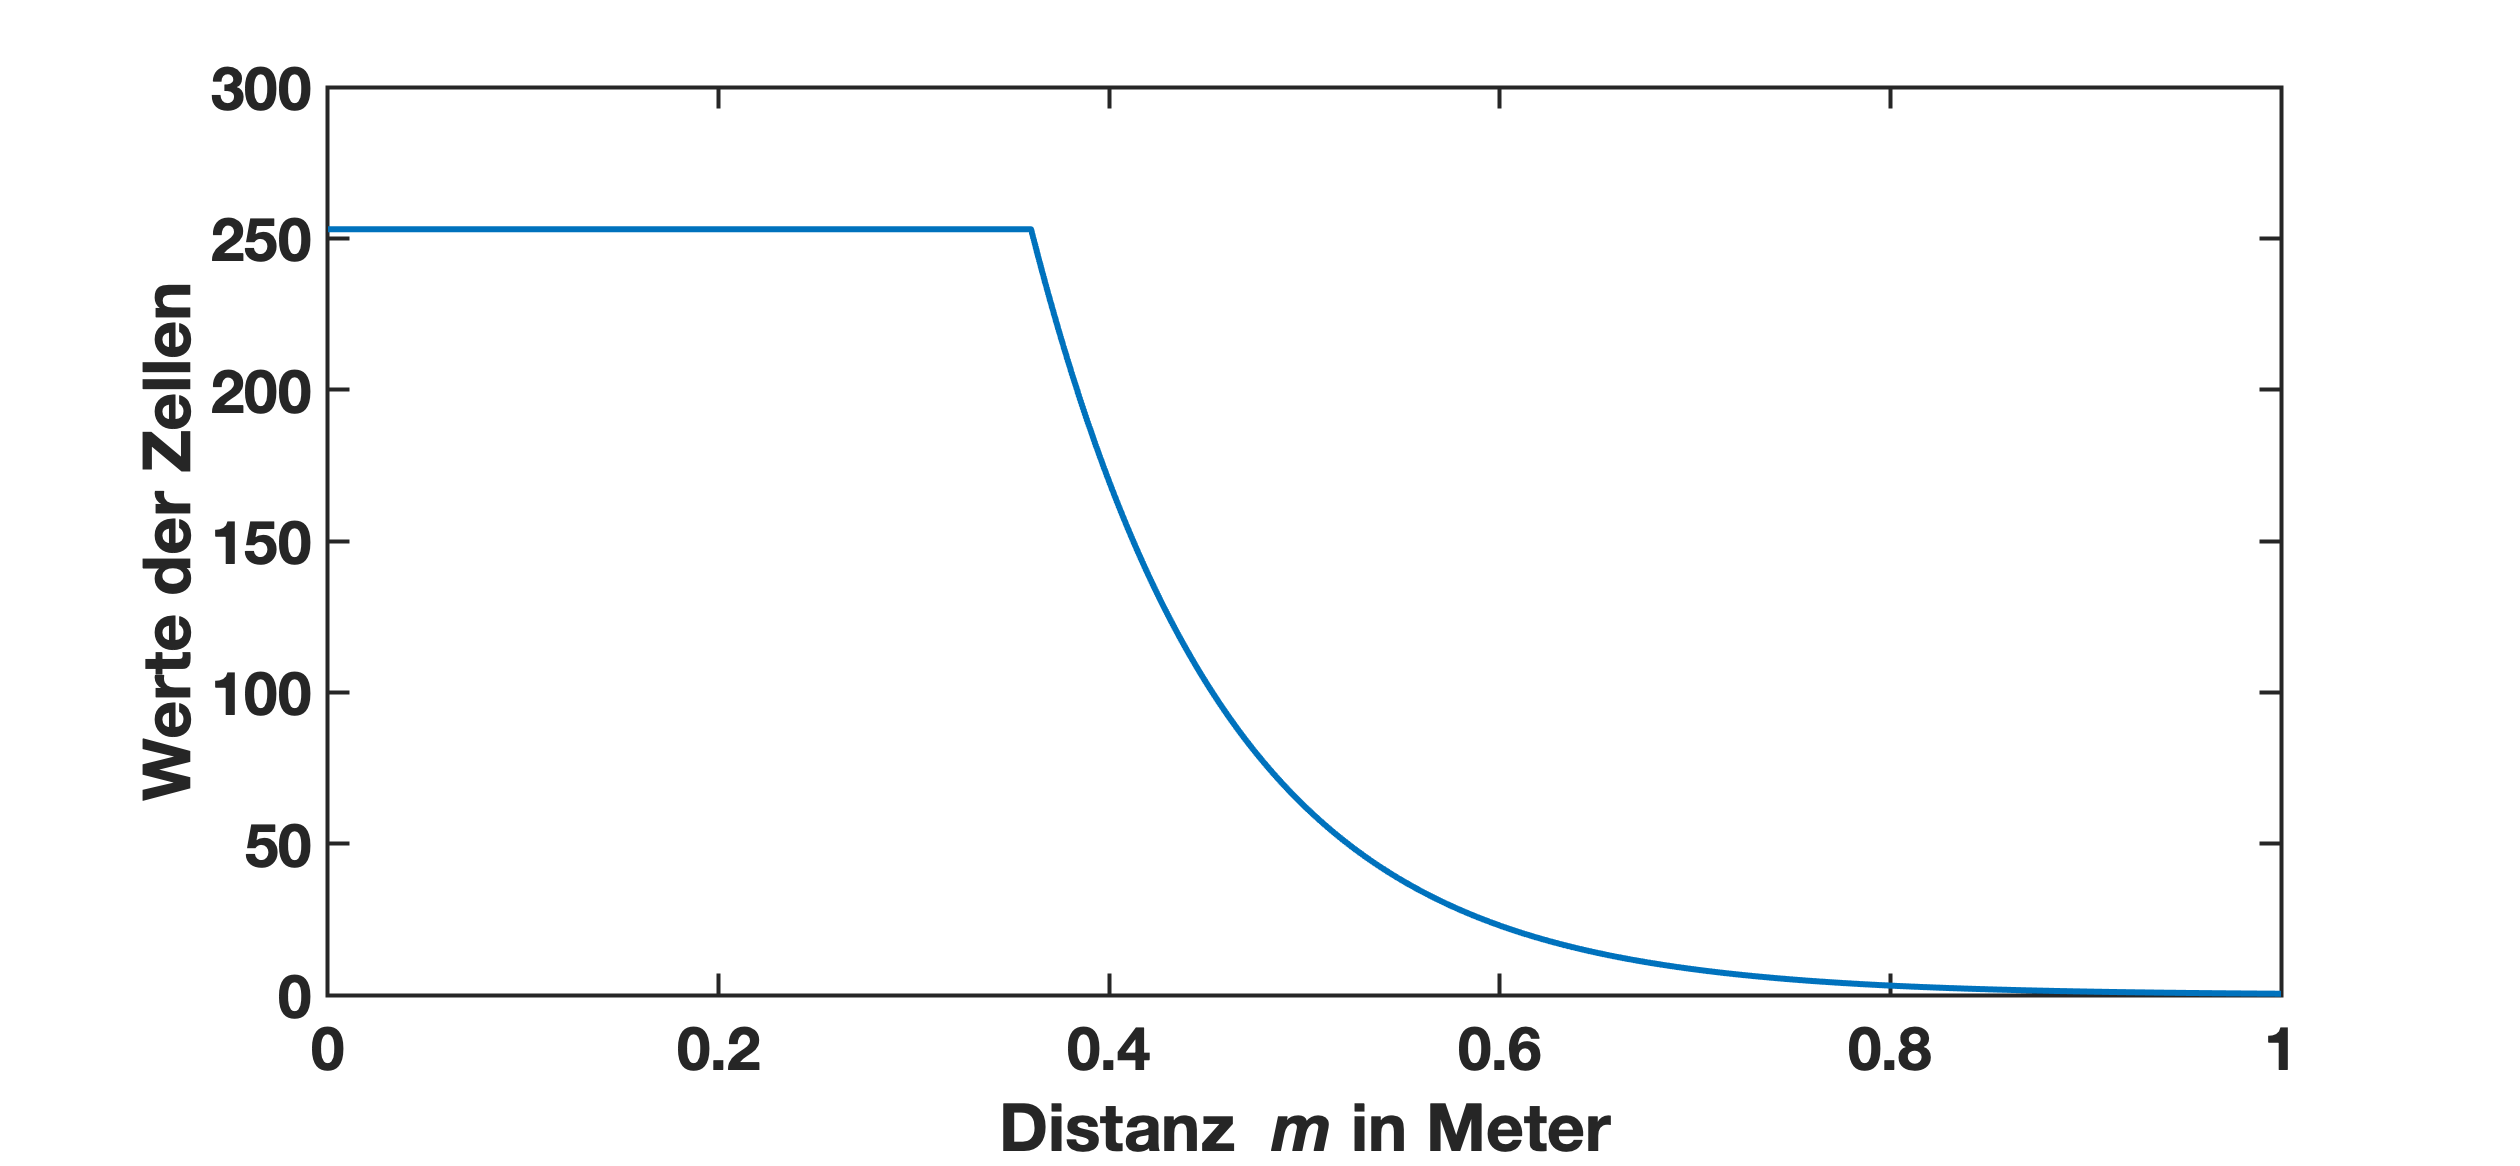
\includegraphics[width=0.8\textwidth]{Bilder/costmap_verteilung.png}
		    		\caption{Verteilung der Werte über die Distanz r. Der Circumscribed Radius liegt bei $\approx0.78\si{m}$ und der Inflation Radius bei $1.0\si{m}$. Die Distanz von der besetzten Zelle $r=0\si{m}$ bis zum inscribed Radius $r=0.36\si{m}$ erhält den Wert 253, die restliche Werteverteilung entspricht dem Funktionsverlauf aus Gleichung \ref{eq: cost} mit den definierten Parametern.} 
		    		\label{fig: costverteilung}
		    	\end{figure}
		    
		    
		    Abbildung \ref{fig: trajektorie} zeigt eine vom Teb Local Planner geplante Trajektorie in einer Costmap. Die Zielpose wurde in Rviz händisch bewusst in unbekanntest Gebiet gelegt, damit deutlich zu erkennen ist, dass die Trajektorie abhängig von den Sicherheitsradien und unbekannten, noch nicht gewichteten, Gebiet ist und diese Parameter in die Planung mit einbezogen werden. In der Abbildung ist die eingegebene Zielpose als grüner Pfeil in unbekanntem Gebiet, die vom Teb Local Planner geplante Trajektorie (rote Pfeile entlang des Inflation Radius), der Roboterumriss des Fahrzeugs als grünes Rechteck und die gewichteten Bereiche der Costmap zu sehen.
		    
		    \begin{figure}[H]
		    	\centering
		    	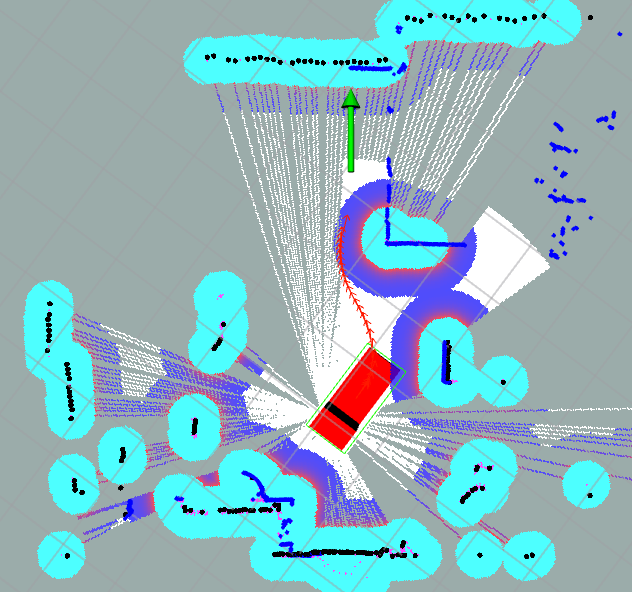
\includegraphics[width=0.8\textwidth]{Bilder/trajektorie.png}
		    	\caption{Darstellung einer Costmap mit eingetragener Trajektorie von oben betrachtet. Anhand der blauen und schwarzen Punkte erkennt man die visualisierten \textit{LaserScan}-Daten, wie bereits in Abbildung xy veranschaulicht. In der Darstellung sind um diese Punkte die Gewichtungen der Costmap farblich markiert. Als Kette aus roten Pfeilen ist die abzufahrende Trajektorie dargestellt. Oben im Zentrum des Bildes repräsentiert ein grüner Pfeil die Roboterzielpose und das grüne Viereck den Roboterumriss. Die vom Roboter ausgehenden Linien und Flächen stellen die Karte aus. \textit{Hector Slam} dar.}
		    	\label{fig: trajektorie}
		    \end{figure}
	    
	    
	    	Neben der Eingabe einer Zielpose in Rviz oder den manuellen Verfahren des Fahrzeugs mit dem Joystick, ist es durch den Explore Lite Knoten möglich eine Zielpose in unbekanntes Gebiet und daraus folgend eine Trajektorie dorthin zu planen. Der Knoten abboniert die von Move Base erstellte Costmap und Veröffentlicht unabhängig vom Benutzer Bewegungsvorgaben, welche wiederum von Move Base zur Planung der Trajektorie genutzt wird. Der Knoten bewertet unbekanntes Gebiet der Costmap als Grenze und versucht diese Grenzen zu erkunden bis kein unbekanntes Gebiet mehr in der Costmap zu finden ist. \cite{explorelite}
		  

		
			
			
					    
		    